\chapter{Benchmark Models and Reference Results}
\label{chap:benchmarks}

%%%%%%%%%%%%%%%%%%%%%%%%%%%%%%%%%%%%%%%%%%%%%%%%%%%%%%%%%%%%%%%%%%%%%%%%%%%%%%%
\section{Motivation}
\label{sec:chap7-motivate}

\begin{itemize}[noitemsep]
  \item identify metrics of interest - eigenvalue, fission, capture rates
  \item match CE MC as closely as possible with deterministic MG theory
  \item understand spatial self-shielding effects in pin-wise MGXS
\end{itemize}


%%%%%%%%%%%%%%%%%%%%%%%%%%%%%%%%%%%%%%%%%%%%%%%%%%%%%%%%%%%%%%%%%%%%%%%%%%%%%%%
\section{Benchmark Configurations}
\label{sec:chap7-benchmarks}

See the isotopic compositions tabulated in App.~\ref{app:beavrs-isotopes}. The \ac{BEAVRS} model~\cite{horelik2013beavrs}.

-add in pitch
-add in mass of grid spacers
-add in axial level


\begin{table}[h!]
  \centering
  \caption[BEAVRS pin cell radii]{Pin cell radii for the \ac{BEAVRS} model.}
  \small
  \label{table:chap7-pin-cell-radii} 
  \vspace{6pt}
  \begin{tabular}{l c}
  \toprule
  \rowcolor{lightgray}
  \multicolumn{1}{c}{\bf Material} &
  \multicolumn{1}{c}{\bf Radius [cm]} \\
  \midrule
  \multicolumn{2}{c}{\bf Fuel Pin} \\
  \midrule
  Fuel &  0.39218 \\
  Helium & 0.40005 \\
  Zircaloy & 0.45720 \\
  \midrule
  \multicolumn{2}{c}{\bf Empty Guide Tube\footnotemark} \\
  \midrule
  Borated Water & 0.56134 \\
  Zircaloy & 0.60198 \\
  \midrule
  \multicolumn{2}{c}{\bf Instrument Tube} \\
  \midrule
  Air & 0.43688 \\
  Zircaloy & 0.48387 \\
  Borated Water & 0.56134 \\
  Zircaloy & 0.60198 \\
  \midrule
  \multicolumn{2}{c}{\bf Burnable Poison\footnotemark} \\
  \midrule
  Air & 0.21400 \\
  Stainless Steel & 0.23051 \\
  Air & 0.24130 \\
  Borosilicate Glass & 0.42672 \\
  Air & 0.43688 \\
  Stainless Steel & 0.48387 \\
  Borated Water & 0.56134 \\
  Zircaloy & 0.60198 \\
  \bottomrule
\end{tabular}
\end{table}

\addtocounter{footnote}{-2}
\stepcounter{footnote}\footnotetext{The control rod guide tube geometry above the dashpot.}
\stepcounter{footnote}\footnotetext{The burnable poison geometry above the dashpot.}

\begin{figure}[h!]
\centering
\begin{subfigure}{.5\textwidth}
  \centering
  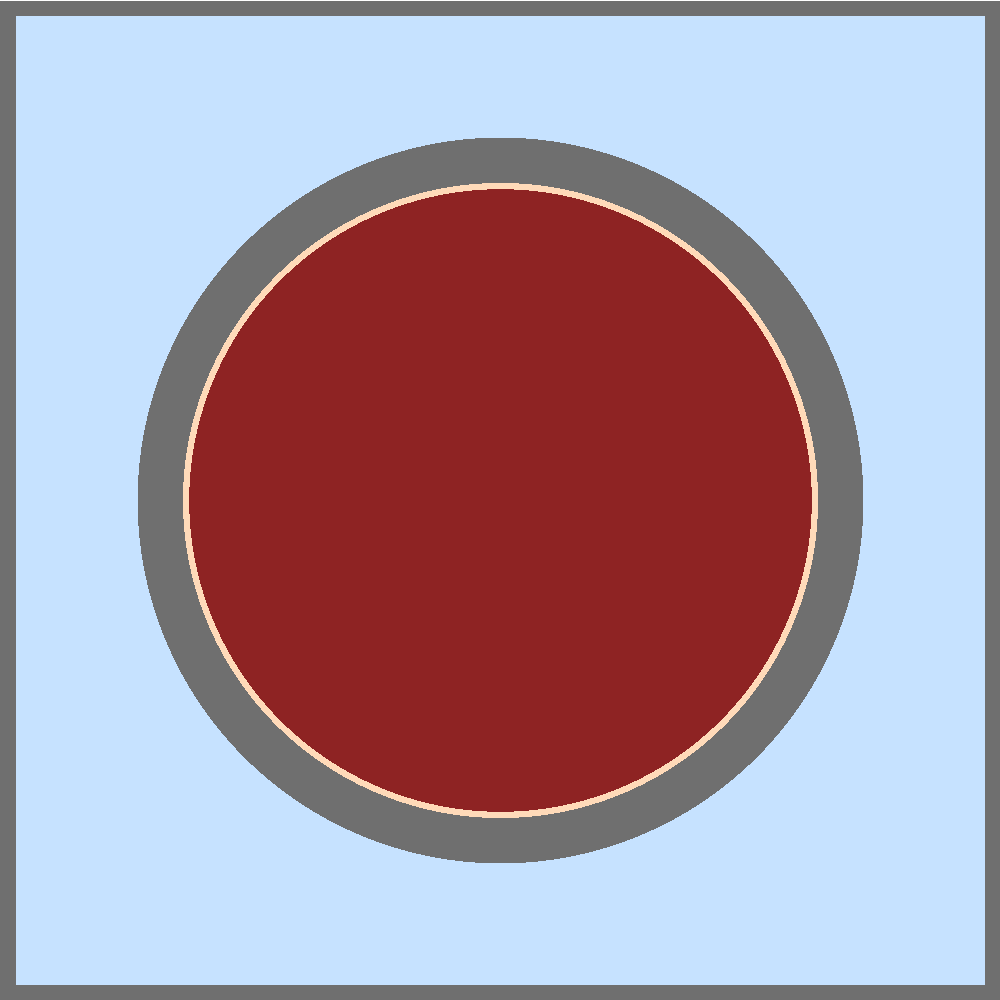
\includegraphics[width=0.9\linewidth]{figures/benchmarks/fuel-pin-16}
  \caption{}
  \label{fig:chap7-pin-1.6}
\end{subfigure}%
\begin{subfigure}{.5\textwidth}
  \centering
  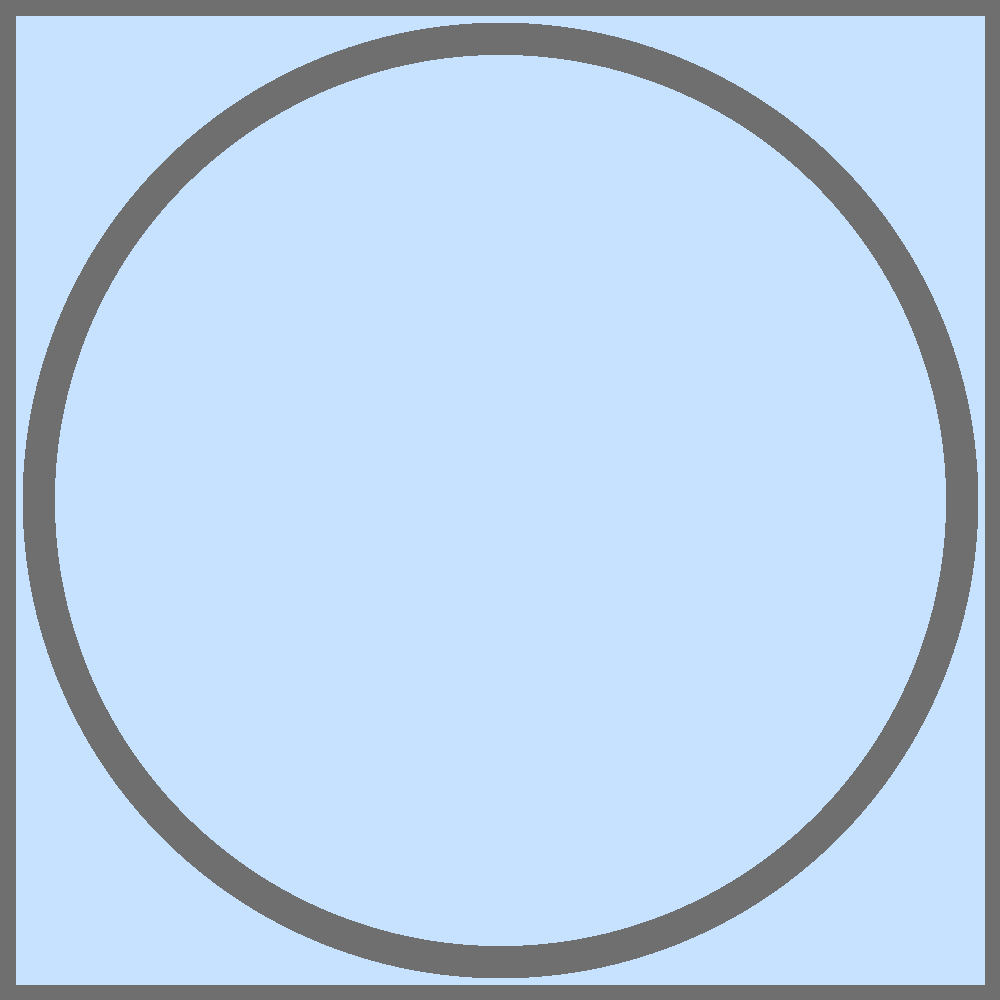
\includegraphics[width=0.9\linewidth]{figures/benchmarks/guide-tube}
  \caption{}
  \label{fig:chap7-pin-3.1}
\end{subfigure}
\begin{subfigure}{.5\textwidth}
  \centering
  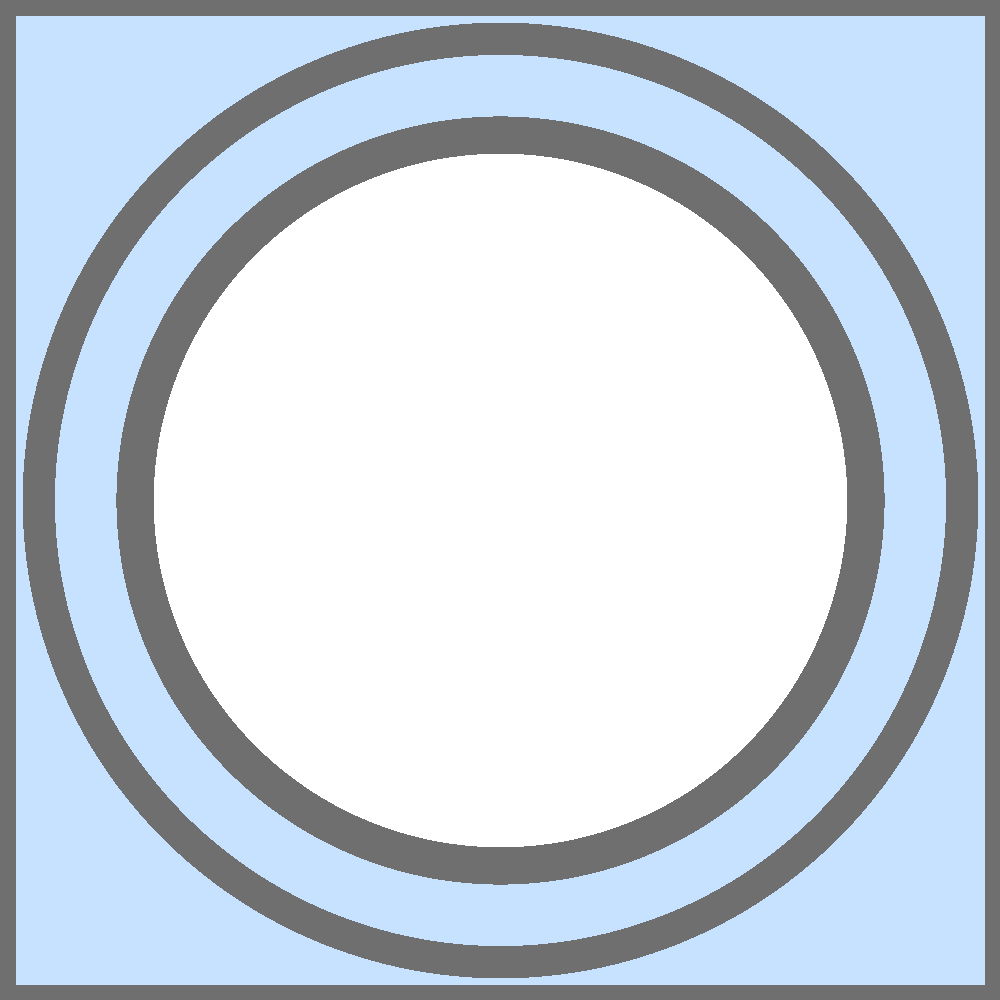
\includegraphics[width=0.9\linewidth]{figures/benchmarks/instr-tube}
  \caption{}
  \label{fig:chap7-guide-tube}
\end{subfigure}%
\begin{subfigure}{.5\textwidth}
  \centering
  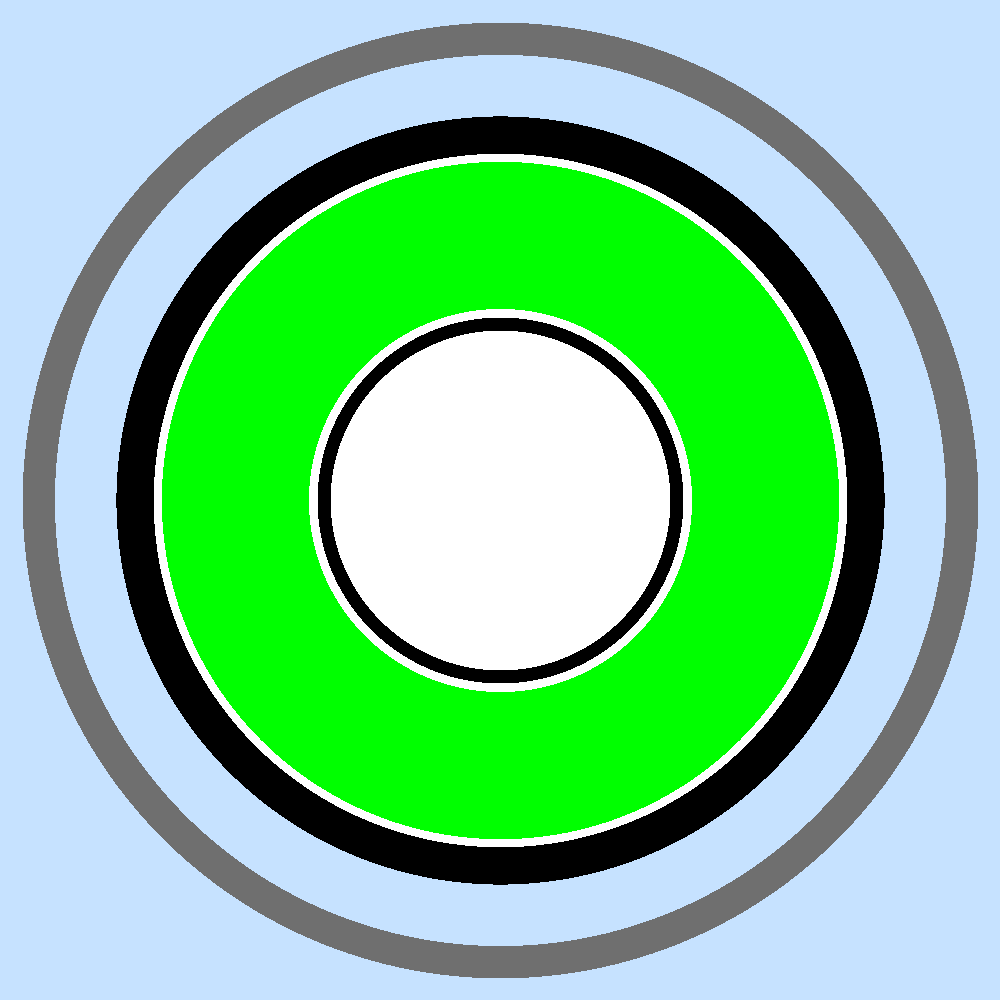
\includegraphics[width=0.9\linewidth]{figures/benchmarks/burn-abs}
  \caption{}
  \label{fig:chap7-instr-tube}
\end{subfigure}%
\caption[BEAVRS pin cell geometries]{1.6\% enriched fuel pin (a), control rod guide tube (b), instrument tube (c) and burnable poison (d). Blue -- borated water, red -- UO$_2$ fuel, gray -- zircaloy, brown -- helium, white -- air, green -- borosolicate glass; black -- stainless steel.}
\label{fig:chap7-pin-cells}
\end{figure}

%\begin{figure}[h!]
%  \centering
%  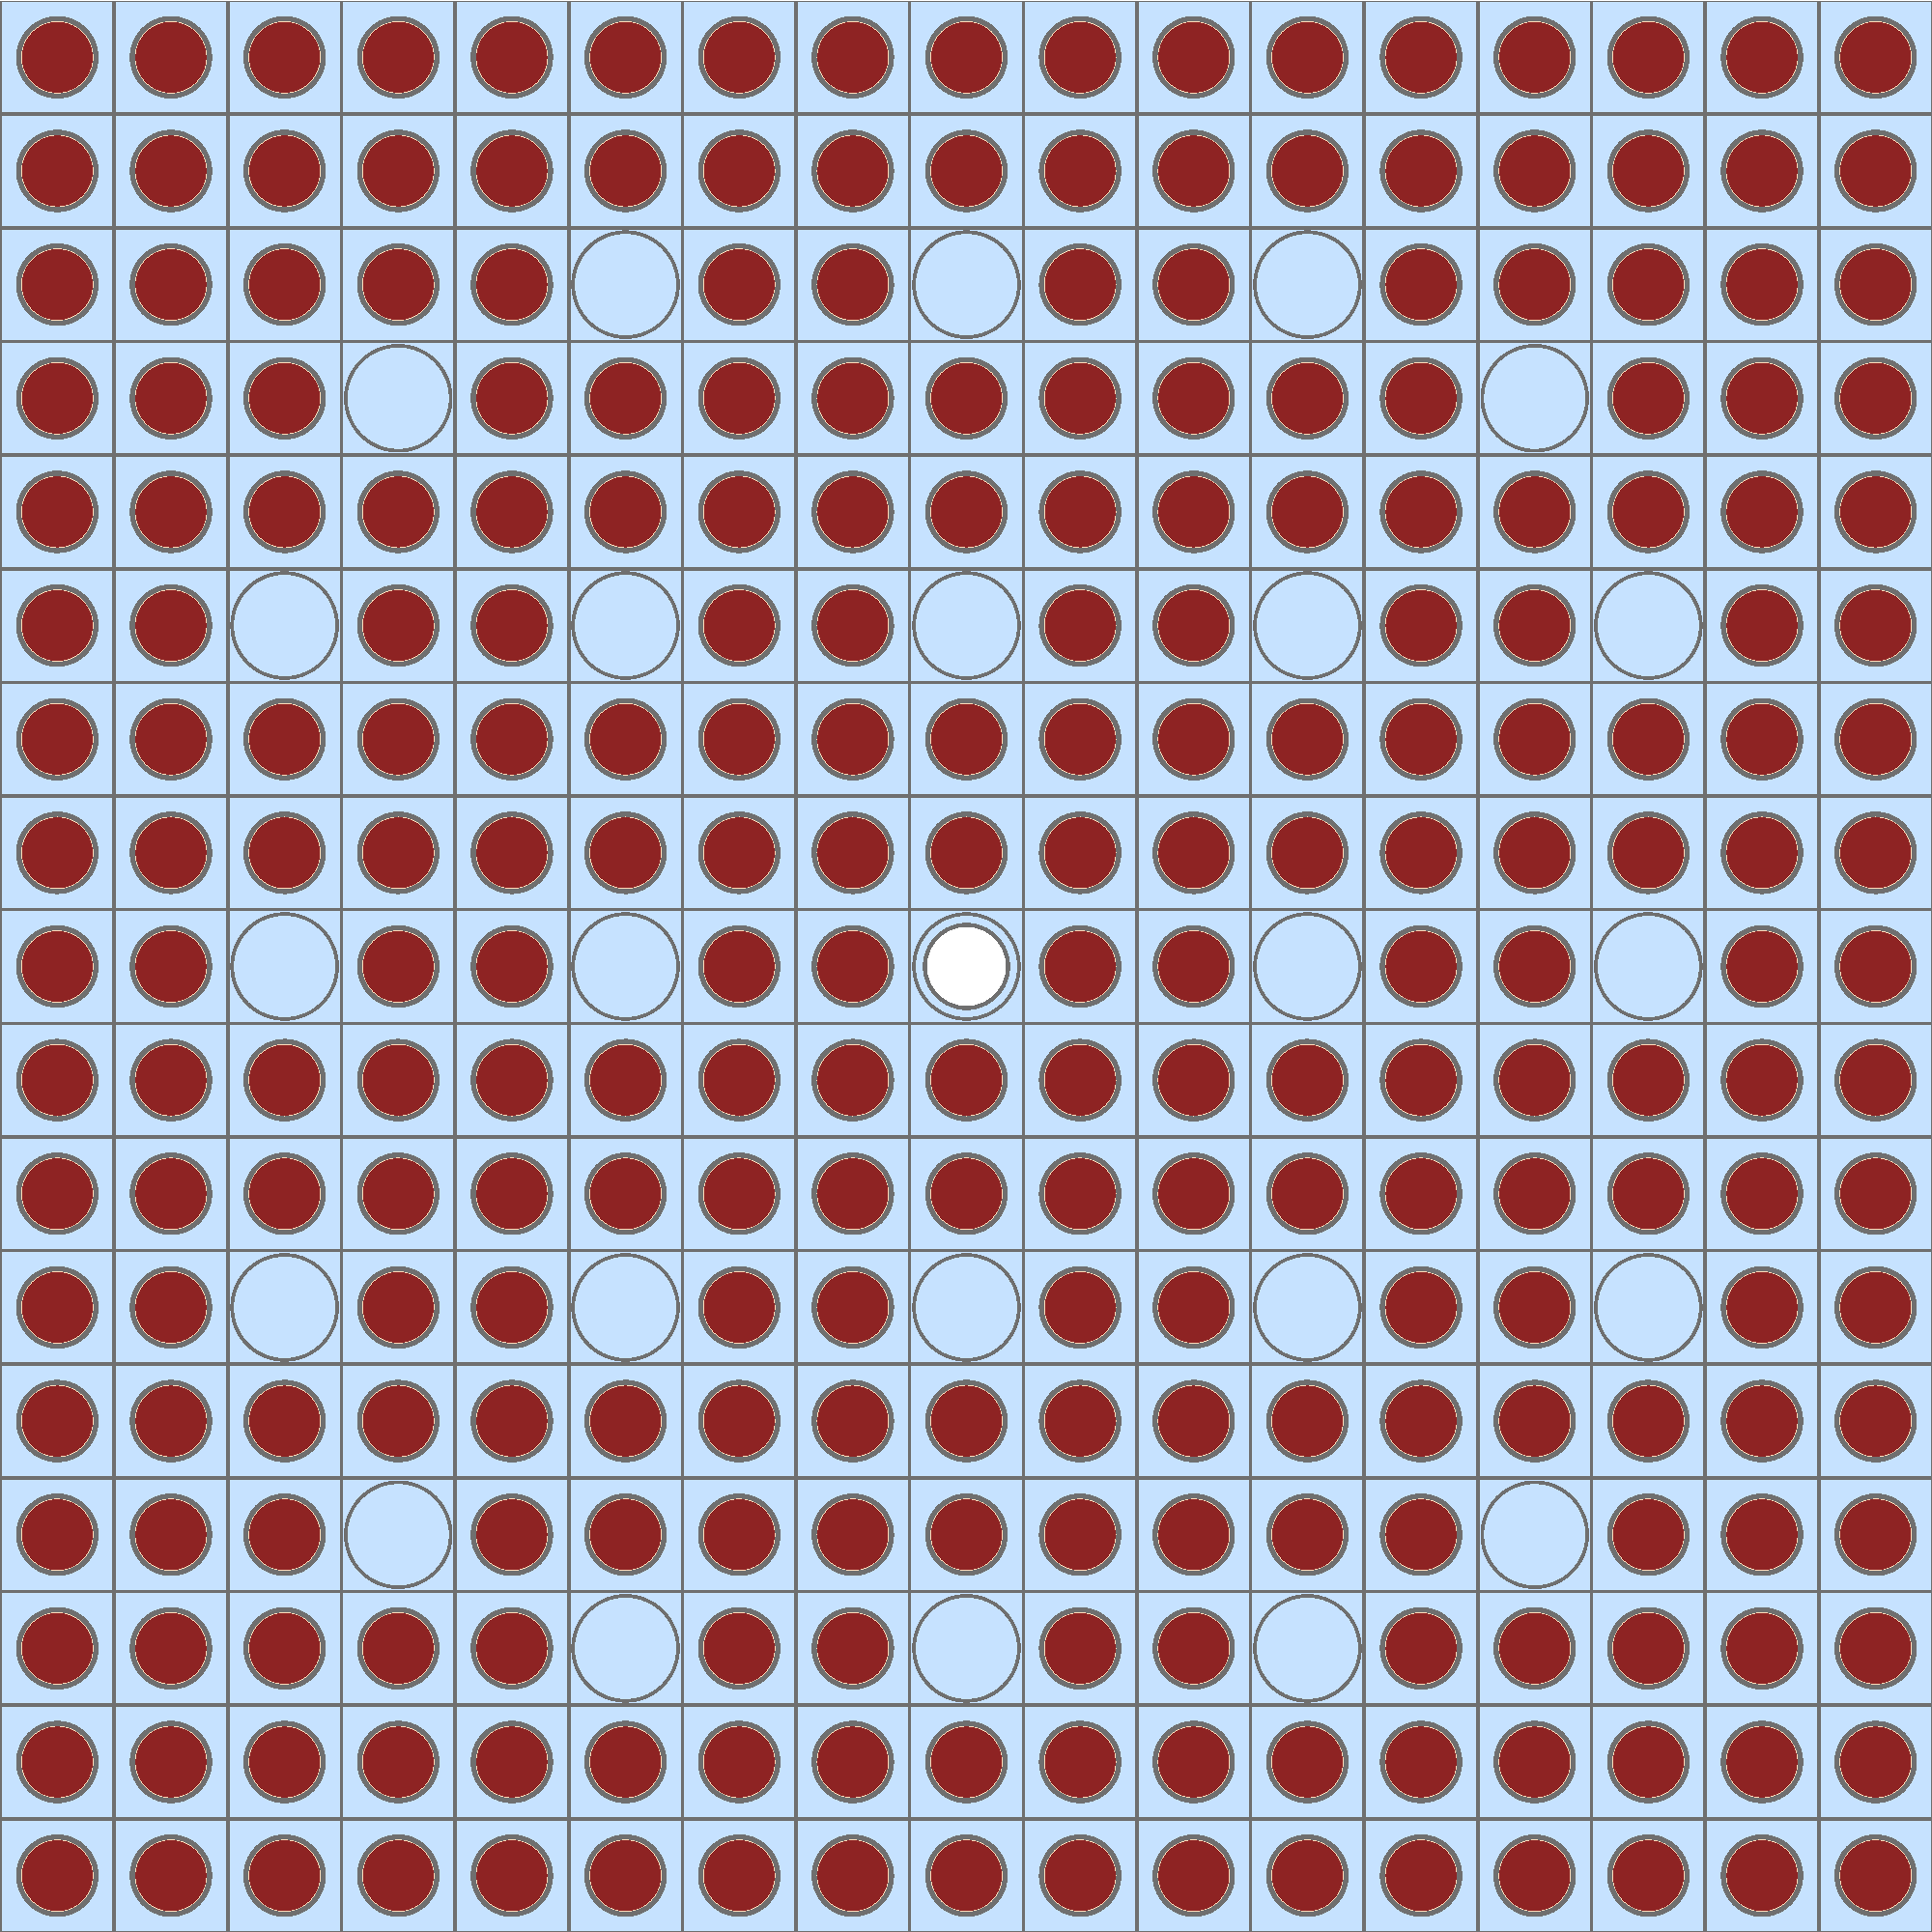
\includegraphics[width=0.65\linewidth]{figures/benchmarks/assembly-16}
%\caption[BEAVRS 1.6\% enriched assembly]{Whoa}
%\label{fig:chap7-assm-16}
%\end{figure}

\begin{figure}[h!]
  \centering
  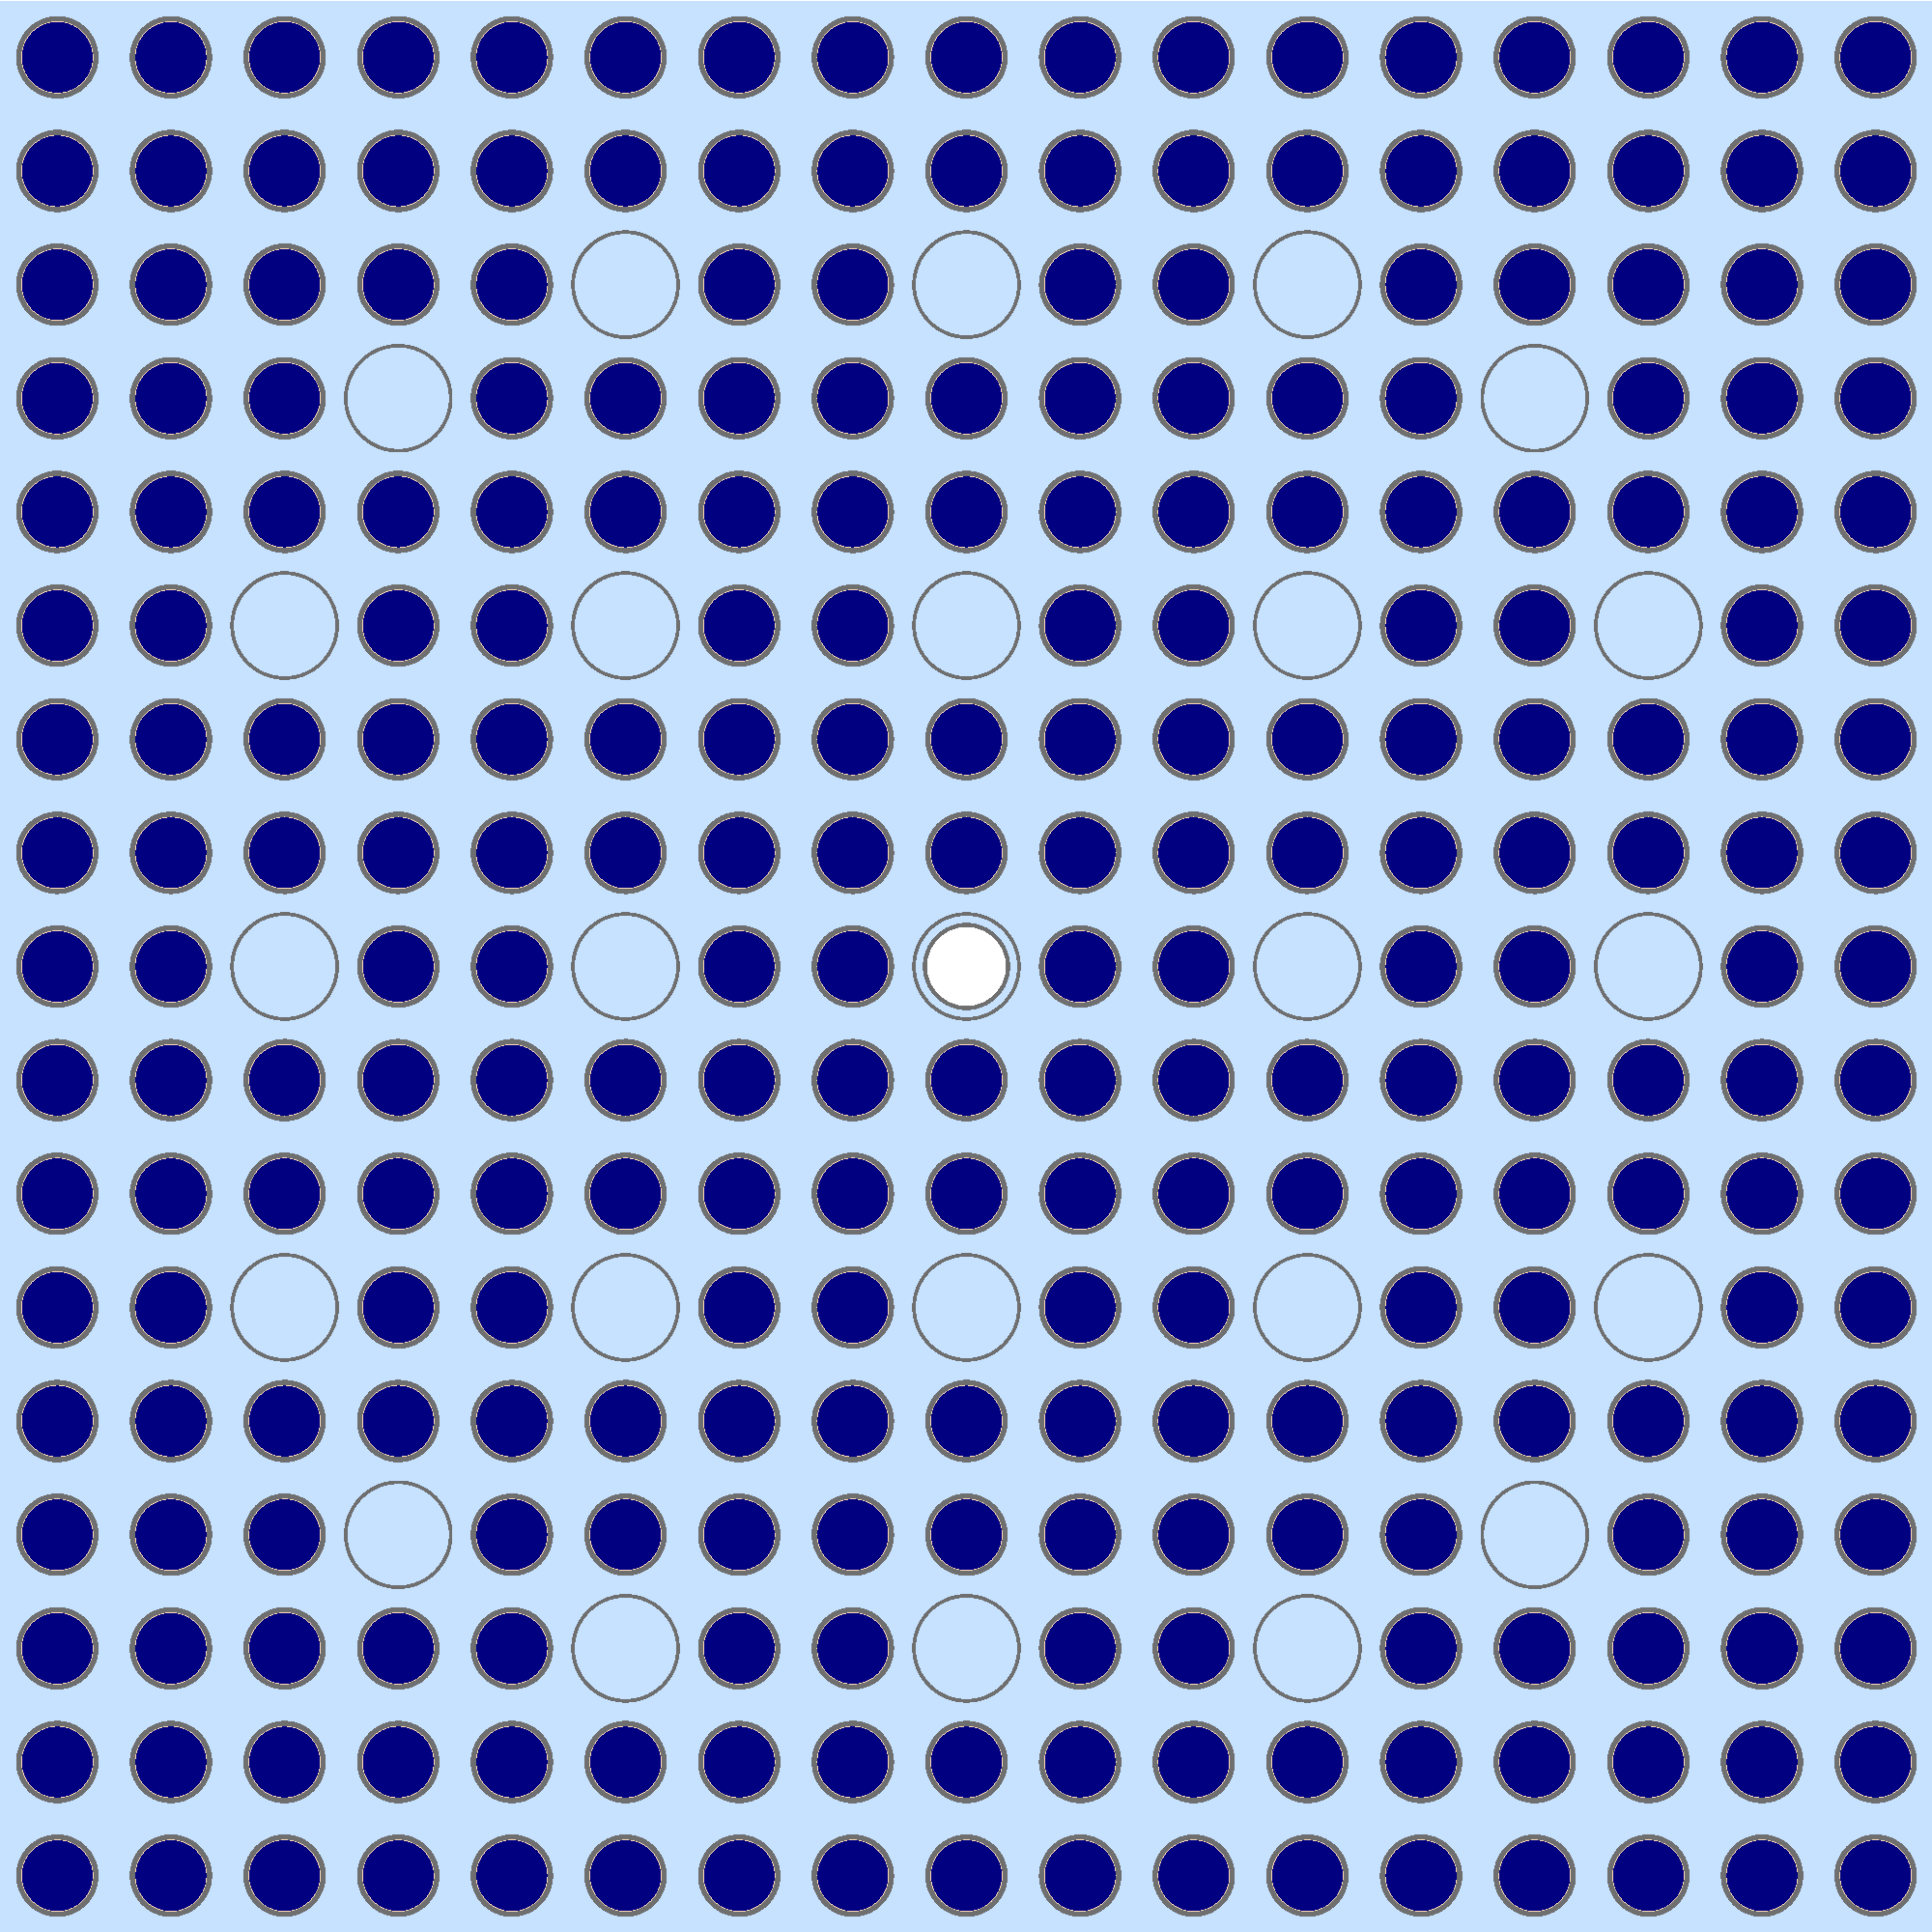
\includegraphics[width=0.65\linewidth]{figures/benchmarks/assembly-31}
\caption[BEAVRS 3.1\% enriched assembly]{Whoa}
\label{fig:chap7-assm-31}
\end{figure}

\begin{figure}[h!]
  \centering
  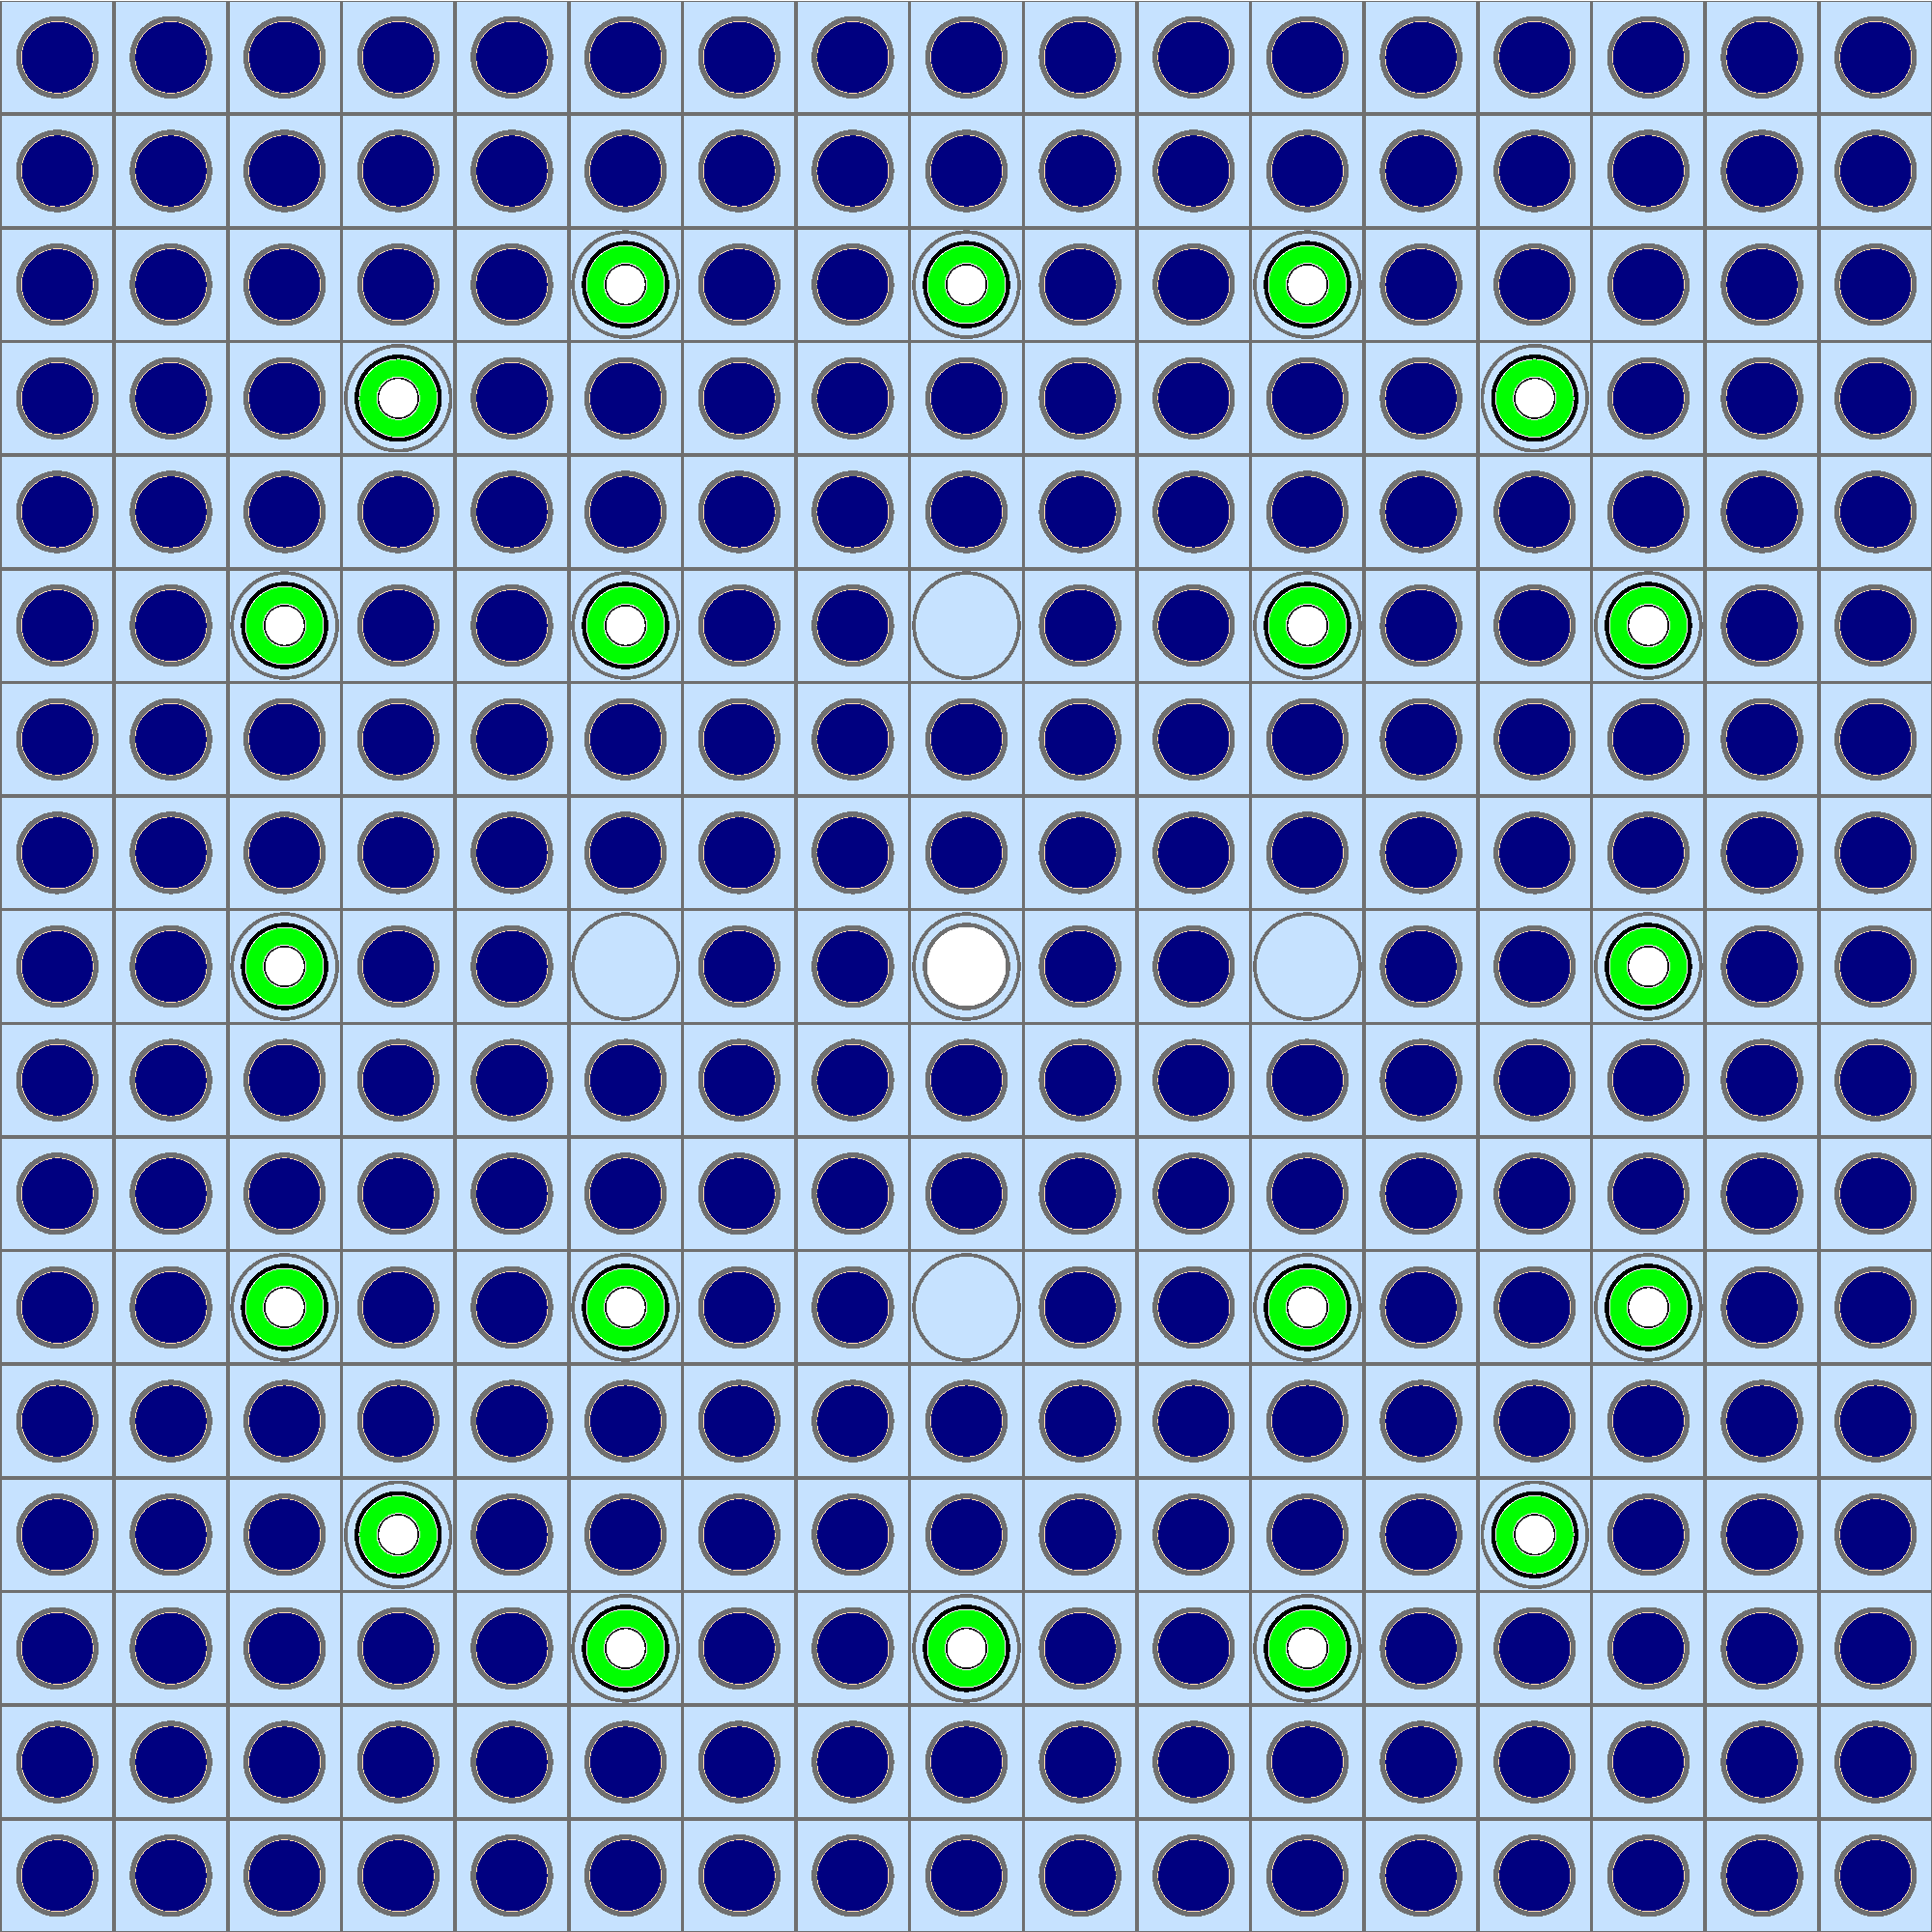
\includegraphics[width=0.65\linewidth]{figures/benchmarks/assembly-31-20BAs}
\caption[BEAVRS 3.1\% enriched assembly with 20 \ac{BP}s]{Whoa}
\label{fig:chap7-assm-31-20BAs}
\end{figure}

\begin{figure}[h!]
  \centering
  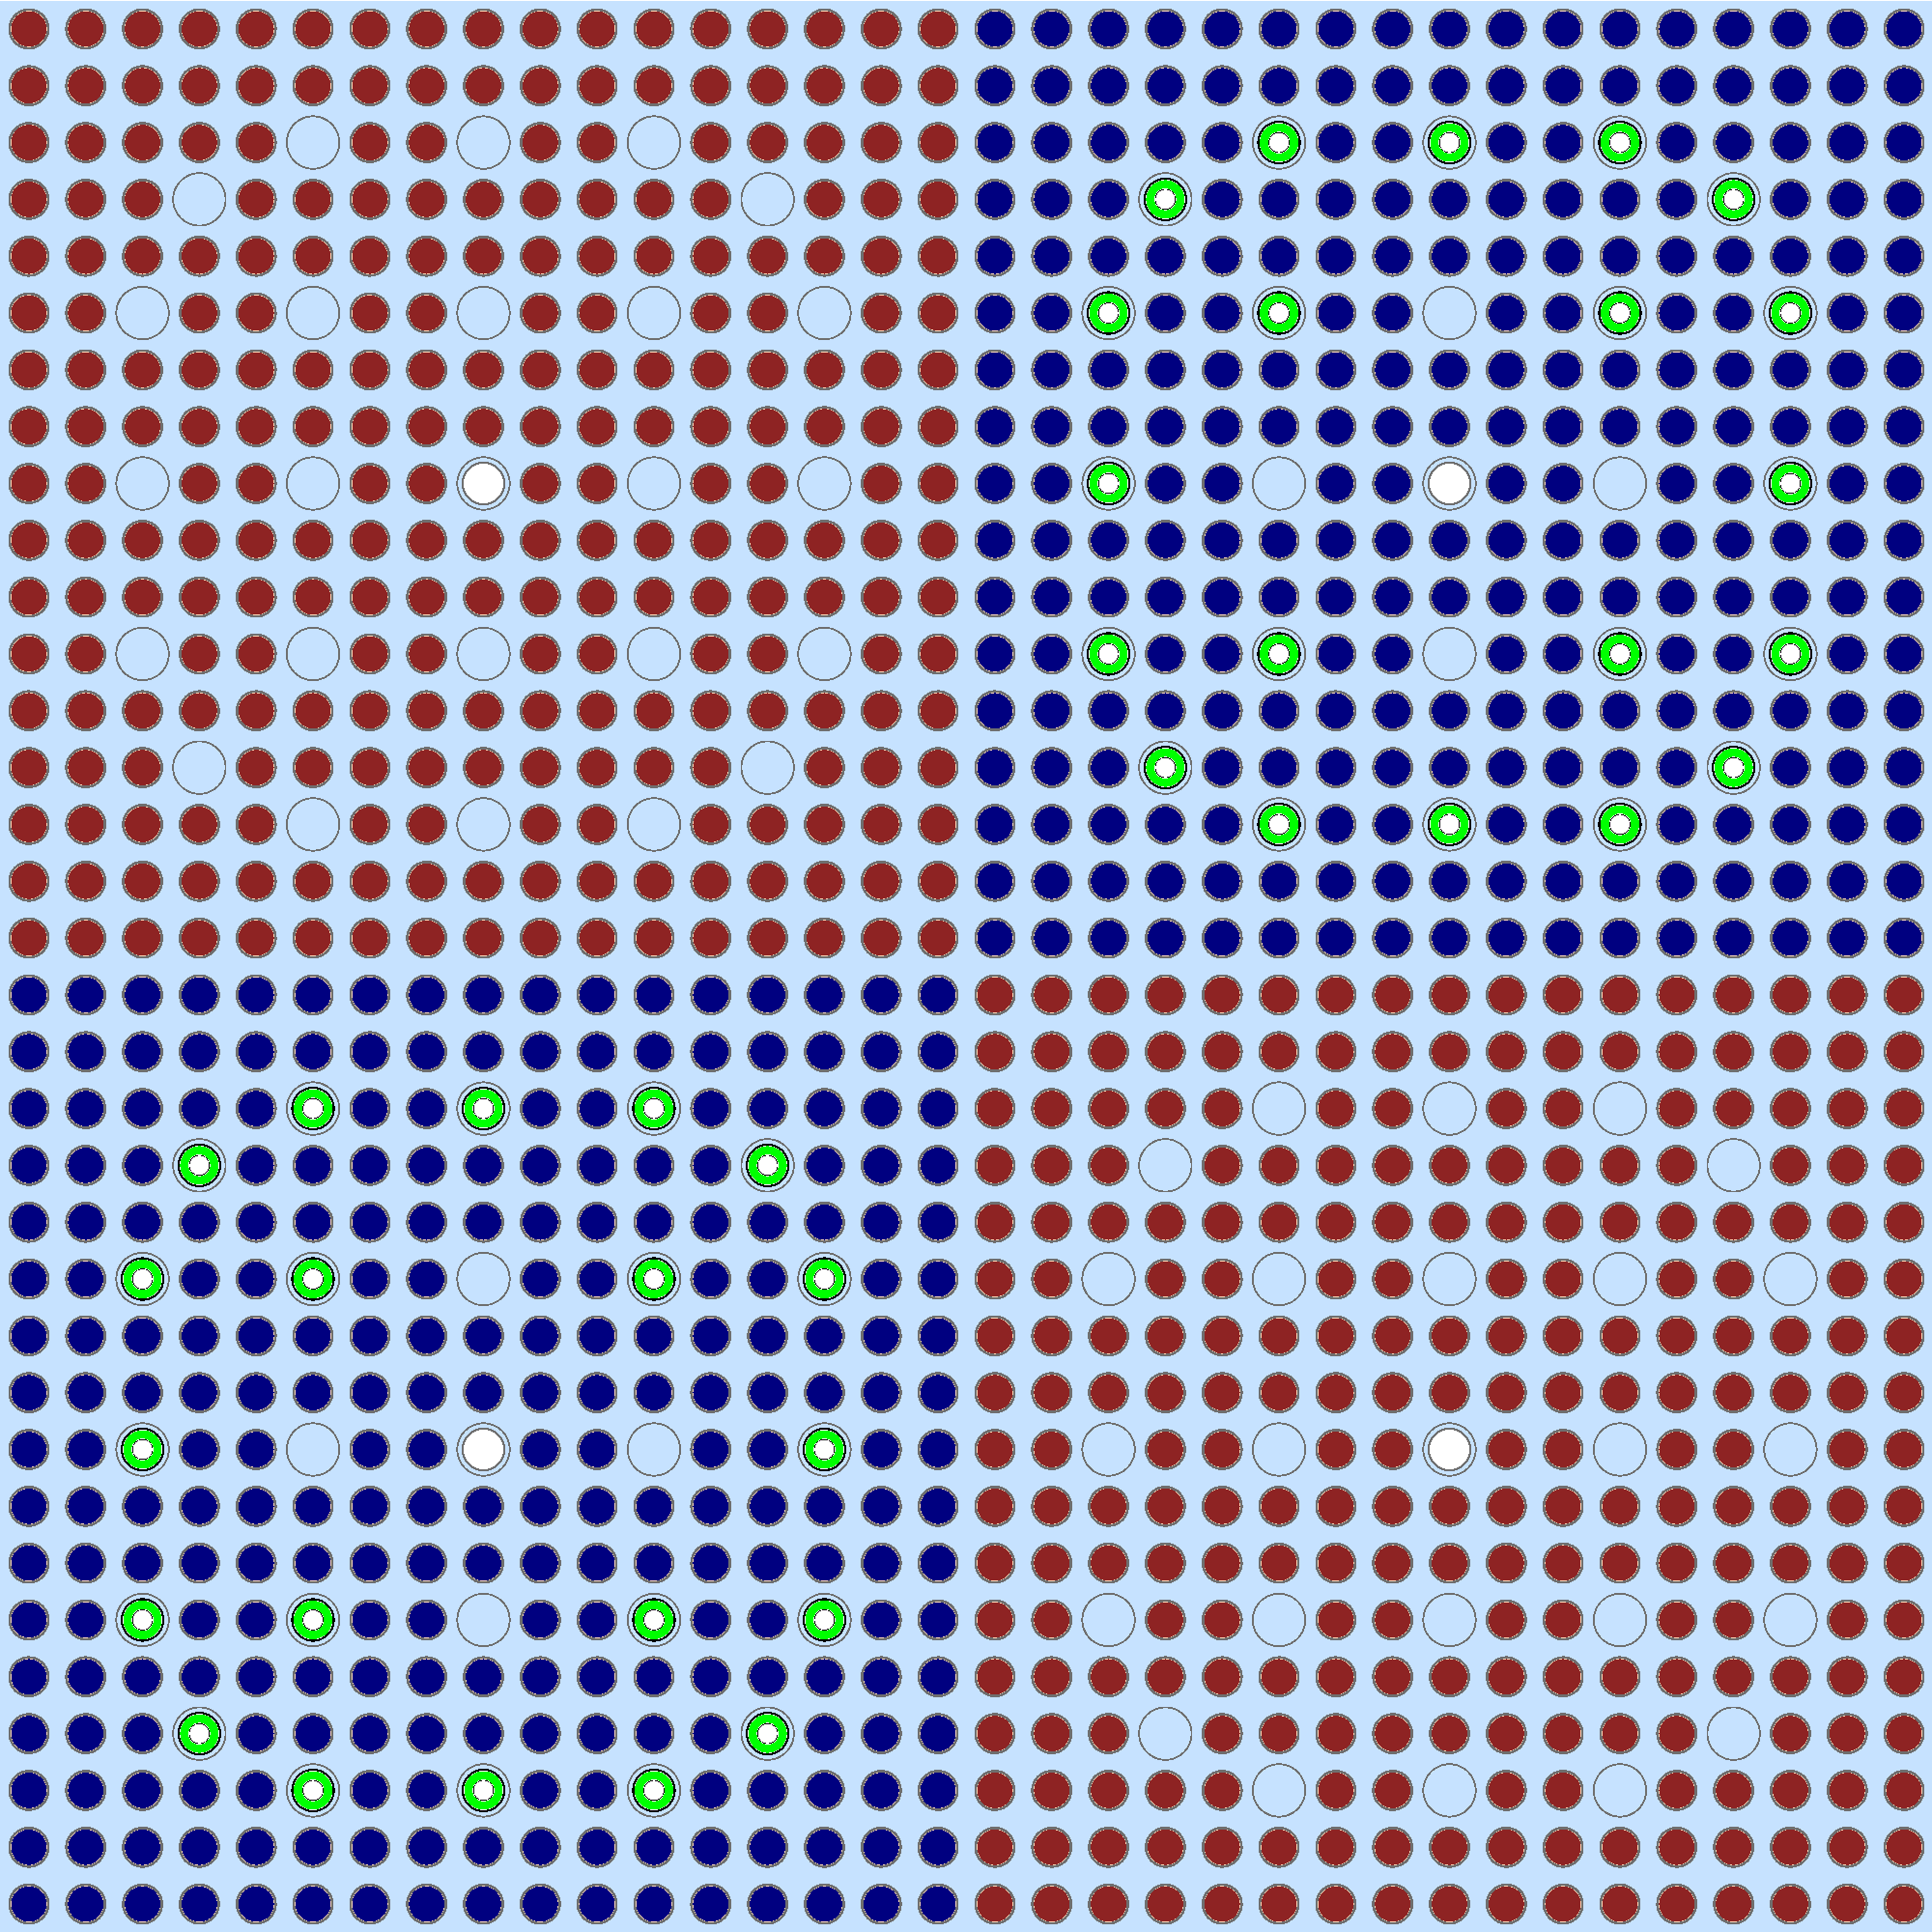
\includegraphics[width=0.65\linewidth]{figures/benchmarks/2x2}
\caption[A 2$\times$2 colorset of BEAVRS assemblies]{Whoa}
\label{fig:chap7-2x2}
\end{figure}

\begin{figure}[h!]
  \centering
  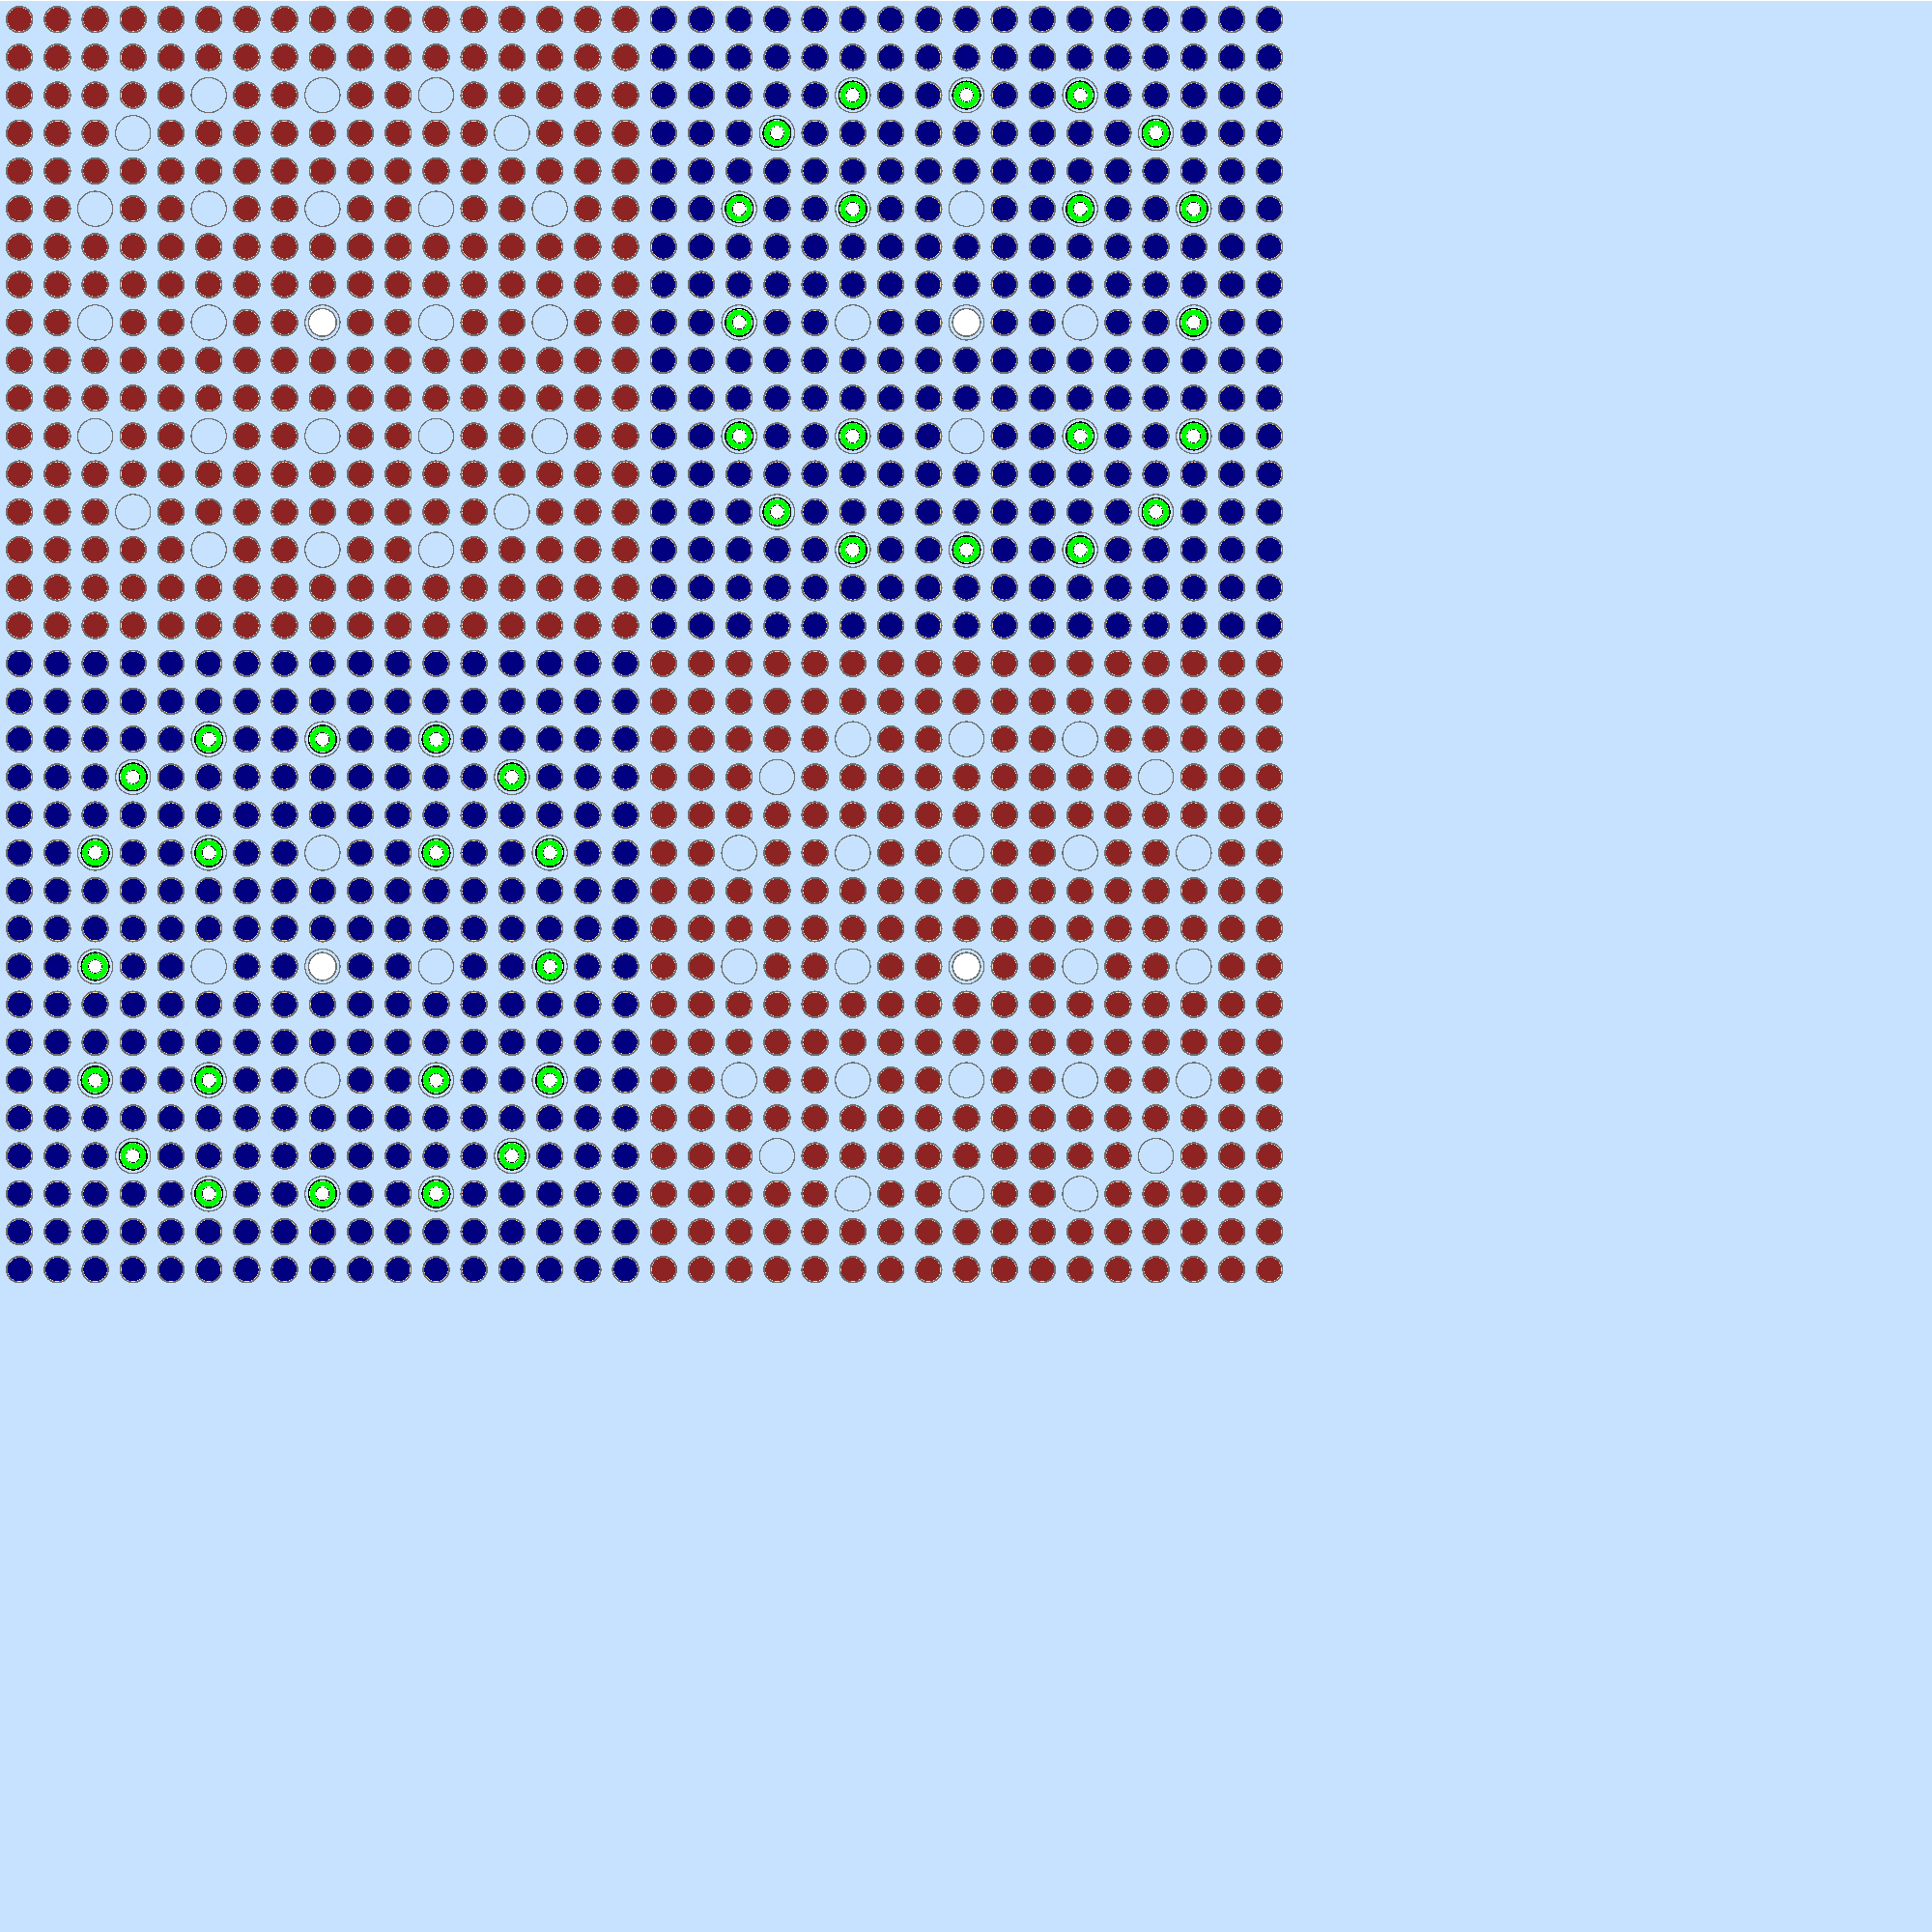
\includegraphics[width=0.65\linewidth]{figures/benchmarks/reflector}
\caption[A reflected 2$\times$2 colorset of BEAVRS assemblies]{Whoa}
\label{fig:chap7-reflector}
\end{figure}

\begin{itemize}[noitemsep]
  \item geometric configuration
  \item isotopics
\end{itemize}

%%%%%%%%%%%%%%%%%%%%%%%%%%%%
\subsection{Fuel Assemblies}
\label{subsec:chap7-fuel-assms}

-figures of each type of sub-component in the geometry
-take from BEAVRS benchmark?

geometric specifications
-fuel pin, radii, clad, gap
-burnable poisons geometry above dashpot
-instrument tube
-\ac{BP}s

isotopics - take table format from Chap. 5 and specs from BEAVRS docs
-fuel
-water
-clad
-gap
-burnable absorber

\subsubsection{1.6\% Enriched Fuel}

-picture of geometry

\subsubsection{2.4\% Enriched Fuel}

-picture of geometry

\subsubsection{2.4\% Enriched Fuel with Burnable Absorbers}

-picture of geometry

\subsection{2$\times$2 Assembly Colorset}

-periodic BCs

\subsection{Reflector Geometry}

-add baffle to benchmark

\subsection{BEAVRS Full Core}


%%%%%%%%%%%%%%%%%%%%%%%%%%%%%%%%%%%%%%%%%%%%%%%%%%%%%%%%%%%%%%%%%%%%%%%%%%%%%%%
\section{Reference Results}
\label{sec:chap7-ref-results}

-mention iso-in-lab

%%%%%%%%%%%%%%%%%%%%%%%%%%%%%%%
\subsection{Source Convergence}
\label{subsec:chap7-src-converge}

-single plot of shannon entropy convergence by batch for each geometry

\begin{figure}[h!]
  \centering
  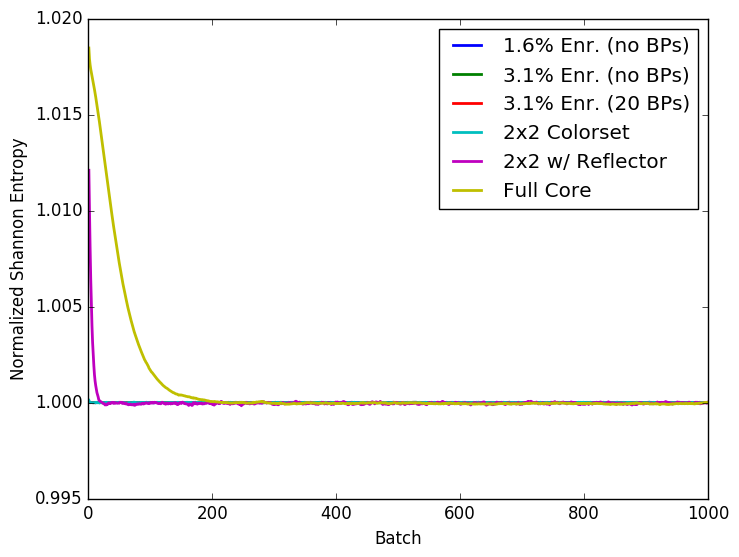
\includegraphics[width=0.9\linewidth]{figures/benchmarks/entropy/entropy-all}
\caption[Shannon entropy source convergence for BEAVRS geometries]{Shannon entropy source convergence for BEAVRS geometries.}
\label{fig:chap7-entropy}
\end{figure}

%\begin{figure}[h!]
%\centering
%\begin{subfigure}{\textwidth}
%  \centering
%  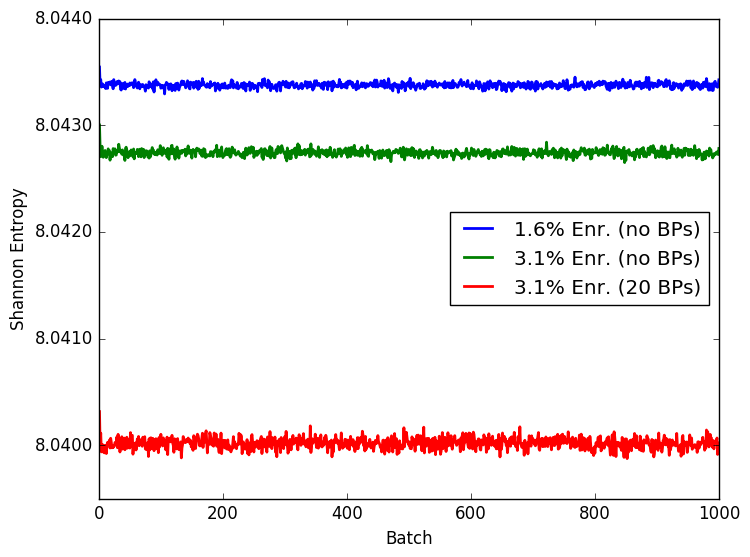
\includegraphics[width=0.9\linewidth]{figures/benchmarks/entropy/entropy-assms}
%  \caption{}
%  \label{fig:chap7-entropy-assms}
%\end{subfigure}
%\begin{subfigure}{\textwidth}
%  \centering
%  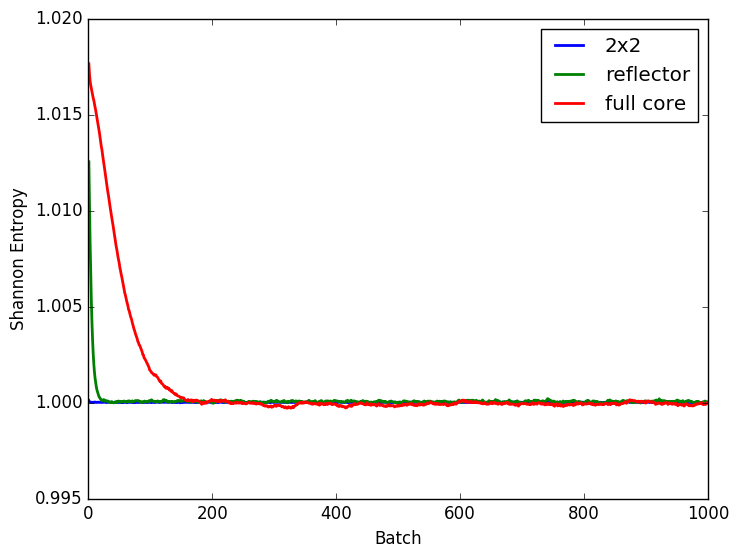
\includegraphics[width=0.9\linewidth]{figures/benchmarks/entropy/entropy-multi-assms}
%  \caption{}
%  \label{fig:chap7-entropy-multi-assms}
%\end{subfigure}%
%\caption[Shannon entropy source convergence for BEAVRS geometries]{Shannon entropy source convergence for BEAVRS geometries.}
%\label{fig:chap7-entropy}
%\end{figure}


%%%%%%%%%%%%%%%%%%%%%%%%
\subsection{Eigenvalues}
\label{subsec:chap7-eigenvalues}

\begin{itemize}[noitemsep]
  \item converged values
  \item convergence by batch
\end{itemize}

\begin{table}[h!]
  \centering
  \caption[Reference $k^{OpenMC}_{eff}$ for heterogeneous benchmarks]{Reference $k^{OpenMC}_{eff}$ for heterogeneous benchmarks.}
  \small
  \label{table:chap7-ref-eigenvalues}
  \vspace{6pt}
  \begin{tabular}{l c}
  \toprule
  \textbf{Benchmark} & \textbf{$k^{OpenMC}_{eff}$} \\
  \midrule
  1.6\% Enriched Assembly (no \ac{BP}s) & 1.00987 $\pm$ 0.00003 \\
  3.1\% Enriched Assembly (no \ac{BP}s) & 1.22344 $\pm$ 0.00003 \\
  3.1\% Enriched Assembly (20 \ac{BP}s) & 1.04530 $\pm$ 0.00003 \\
  2$\times$2 Colorset & 1.03196 $\pm$ 0.00003 \\
  2$\times$2 Colorset w/ Reflector & 0.95462 $\pm$ 0.00003 \\
  \ac{BEAVRS} Full Core & 1.02497 $\pm$ 0.00003 \\
  \bottomrule
\end{tabular}
\end{table}

%%%%%%%%%%%%%%%%%%%%%%%%%%%%%%%%%%%%
\subsection{Pin Power Distributions}
\label{subsec:chap7-pin-powers}

\begin{itemize}[noitemsep]
  \item converged values
  \item convergence by batch
\end{itemize}

\begin{figure}[h!]
\centering
\begin{subfigure}{0.5\textwidth}
  \centering
  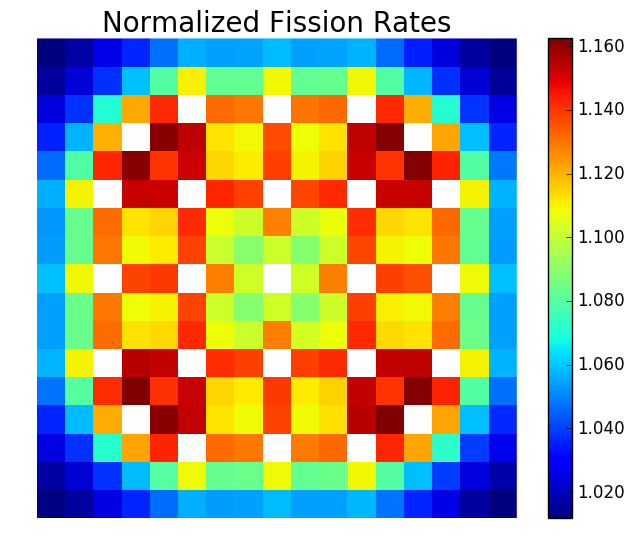
\includegraphics[width=\linewidth]{figures/benchmarks/fission-rates/fiss-mean-fuel-16}
  \caption{}
  \label{fig:chap7-fiss-rate-mean-1.6-assm}
\end{subfigure}%
\begin{subfigure}{0.5\textwidth}
  \centering
  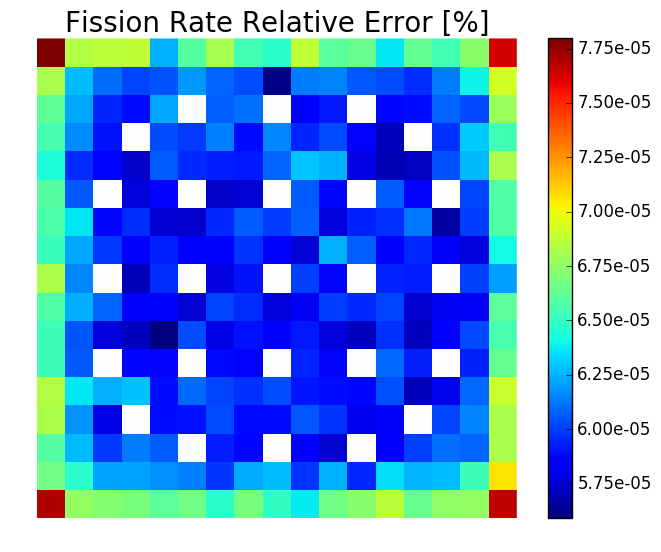
\includegraphics[width=\linewidth]{figures/benchmarks/fission-rates/fiss-rel-err-fuel-16}
  \caption{}
  \label{fig:chap7-fiss-rate-rel-err-1.6-assm}
\end{subfigure}%
\caption[Fission rates for a 1.6\% enriched assembly]{Fission rates for a 1.6\% enriched assembly.}
\label{fig:chap7-fiss-rates-1.6-assm}
\end{figure}

\begin{figure}[h!]
\centering
\begin{subfigure}{0.5\textwidth}
  \centering
  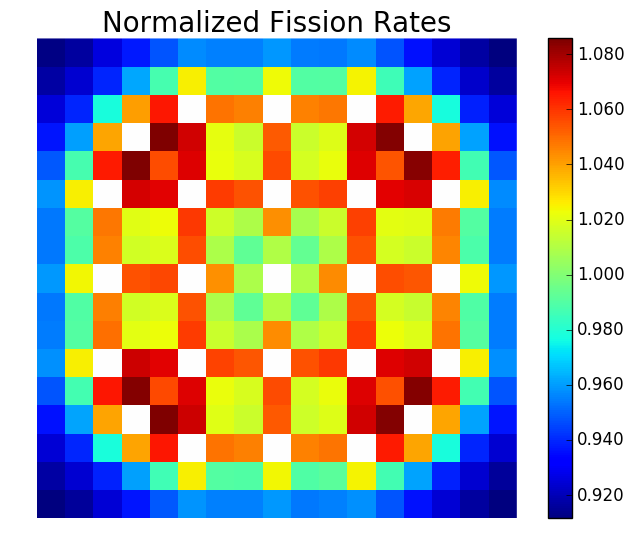
\includegraphics[width=\linewidth]{figures/benchmarks/fission-rates/fiss-mean-fuel-31}
  \caption{}
  \label{fig:chap7-fiss-rate-mean-3.1-assm}
\end{subfigure}%
\begin{subfigure}{0.5\textwidth}
  \centering
  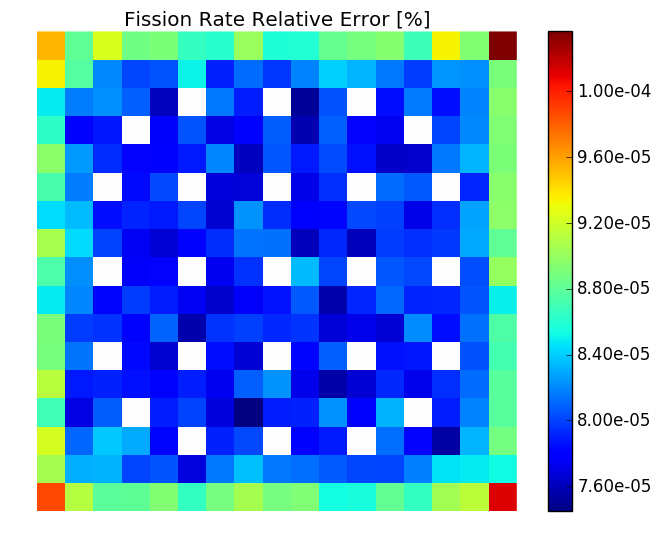
\includegraphics[width=\linewidth]{figures/benchmarks/fission-rates/fiss-rel-err-fuel-31}
  \caption{}
  \label{fig:chap7-fiss-rate-rel-err-3.1-assm}
\end{subfigure}%
\caption[Fission rates for a 3.1\% enriched assembly]{Fission rates for a 3.1\% enriched assembly.}
\label{fig:chap7-fiss-rates-3.1-assm}
\end{figure}

\begin{figure}[h!]
\centering
\begin{subfigure}{0.5\textwidth}
  \centering
  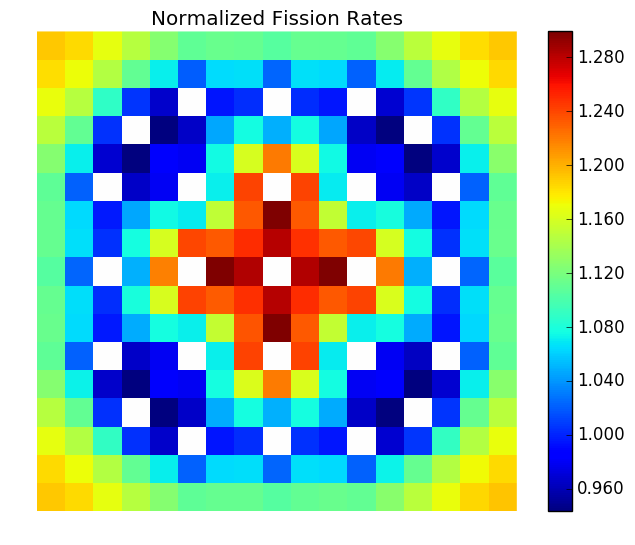
\includegraphics[width=\linewidth]{figures/benchmarks/fission-rates/fiss-mean-fuel-31-20BAs}
  \caption{}
  \label{fig:chap7-fiss-rate-mean-3.1-20BAs-assm}
\end{subfigure}%
\begin{subfigure}{0.5\textwidth}
  \centering
  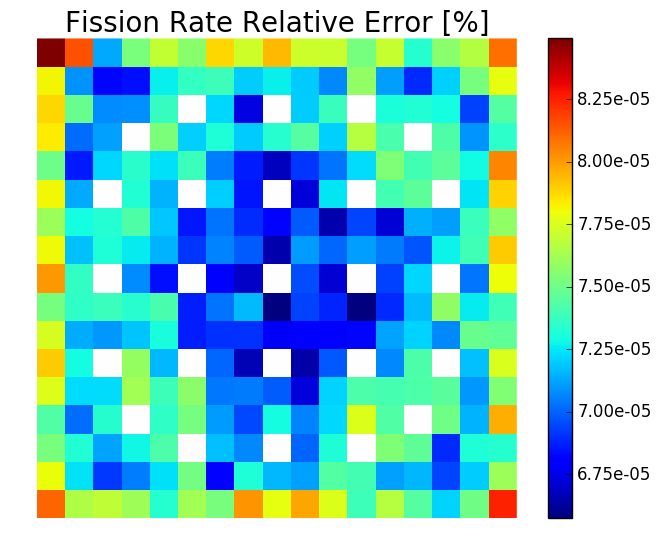
\includegraphics[width=\linewidth]{figures/benchmarks/fission-rates/fiss-rel-err-fuel-31-20BAs}
  \caption{}
  \label{fig:chap7-fiss-rate-rel-err-3.1-20BAs-assm}
\end{subfigure}%
\caption[Fission rates for a 3.1\% enriched assembly with 20 BPs]{Fission rates for a 3.1\% enriched assembly with 20 \ac{BP}s.}
\label{fig:chap7-fiss-rates-3.1-assm-20BAs}
\end{figure}

\begin{figure}[h!]
\centering
\begin{subfigure}{0.5\textwidth}
  \centering
  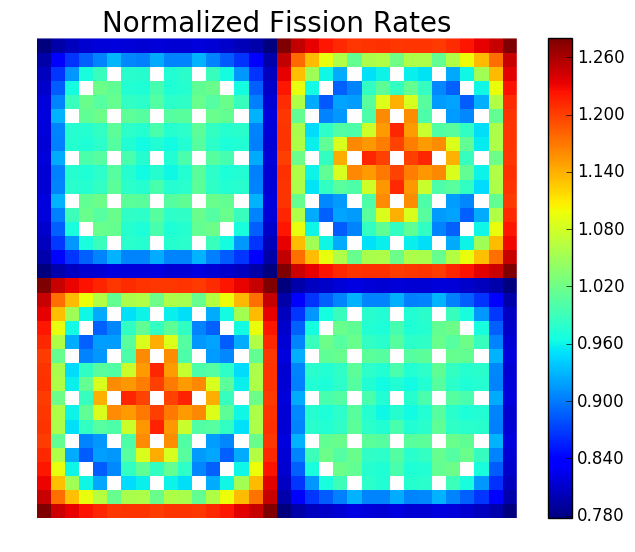
\includegraphics[width=\linewidth]{figures/benchmarks/fission-rates/fiss-mean-2x2}
  \caption{}
  \label{fig:chap7-fiss-rate-mean-2x2}
\end{subfigure}%
\begin{subfigure}{0.5\textwidth}
  \centering
  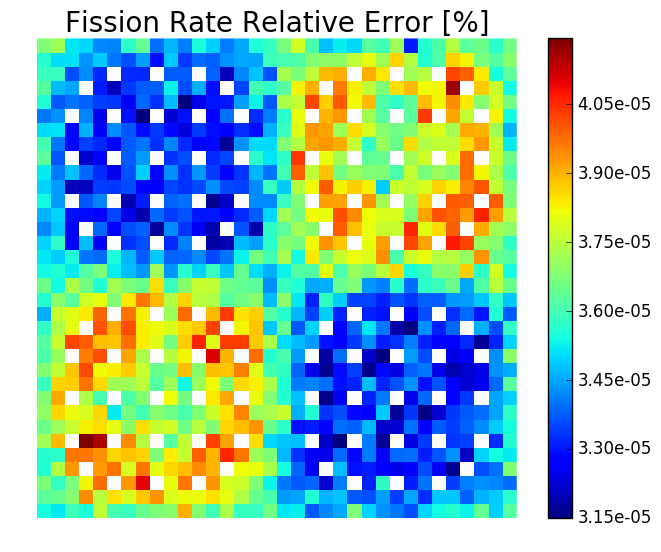
\includegraphics[width=\linewidth]{figures/benchmarks/fission-rates/fiss-rel-err-2x2}
  \caption{}
  \label{fig:chap7-fiss-rate-rel-err-2x2}
\end{subfigure}%
\caption[Fission rates for a 2$\times$2 colorset]{Fission rates for a 2$\times$2 colorset.}
\label{fig:chap7-fiss-rates-2x2}
\end{figure}

\begin{figure}[h!]
\centering
\begin{subfigure}{0.5\textwidth}
  \centering
  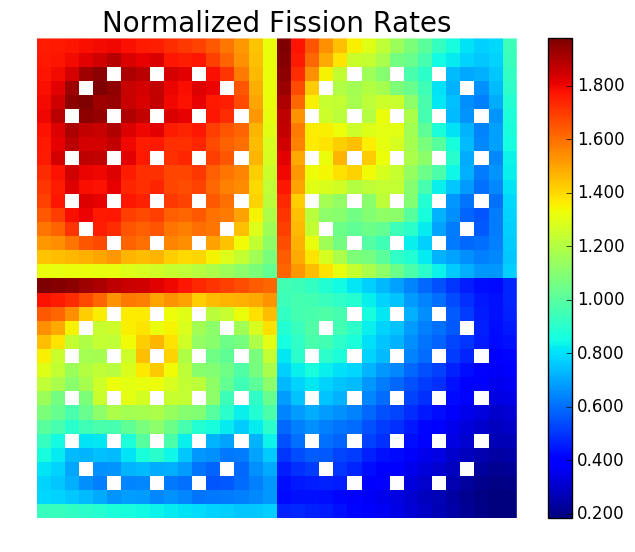
\includegraphics[width=\linewidth]{figures/benchmarks/fission-rates/fiss-mean-reflector}
  \caption{}
  \label{fig:chap7-fiss-rate-mean-reflector}
\end{subfigure}%
\begin{subfigure}{0.5\textwidth}
  \centering
  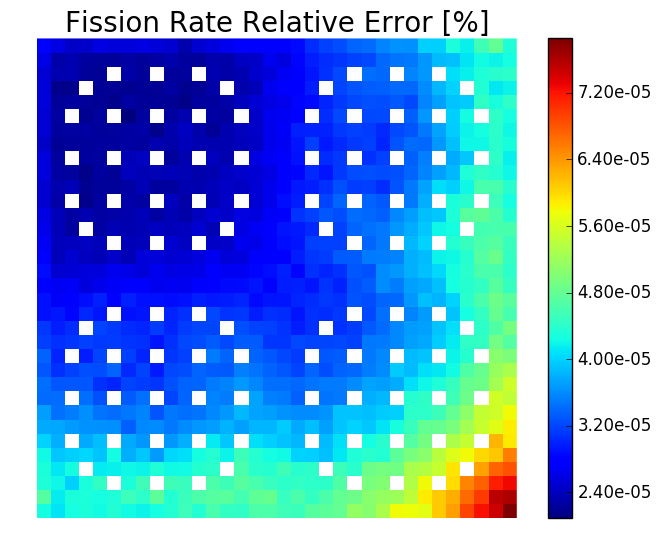
\includegraphics[width=\linewidth]{figures/benchmarks/fission-rates/fiss-rel-err-reflector}
  \caption{}
  \label{fig:chap7-fiss-rate-rel-err-reflector}
\end{subfigure}%
\caption[Fission rates for a 2$\times$2 colorset with a reflector]{Fission rates for a 2$\times$2 colorset with a reflector.}
\label{fig:chap7-fiss-rates-2x2}
\end{figure}

\begin{figure}[h!]
\centering
\begin{subfigure}{0.5\textwidth}
  \centering
  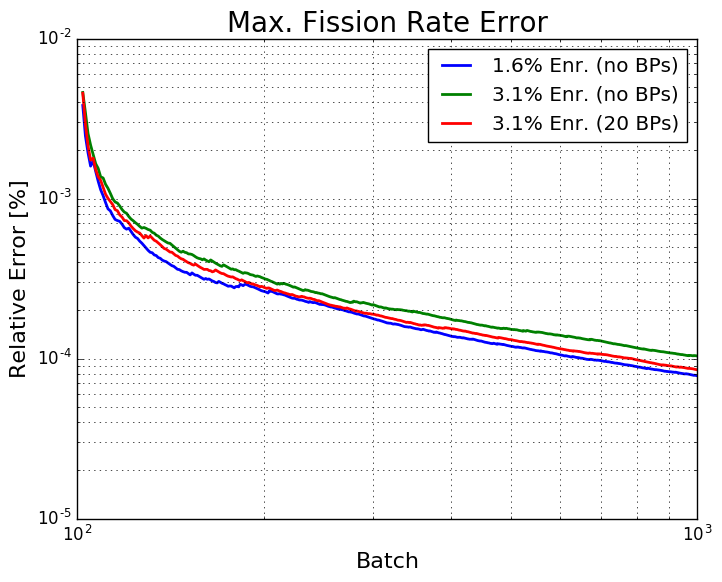
\includegraphics[width=\linewidth]{figures/benchmarks/fission-rates/fiss-conv-max-assms}
  \caption{}
  \label{fig:chap7-fiss-rate-max-conv-assms}
\end{subfigure}%
\begin{subfigure}{0.5\textwidth}
  \centering
  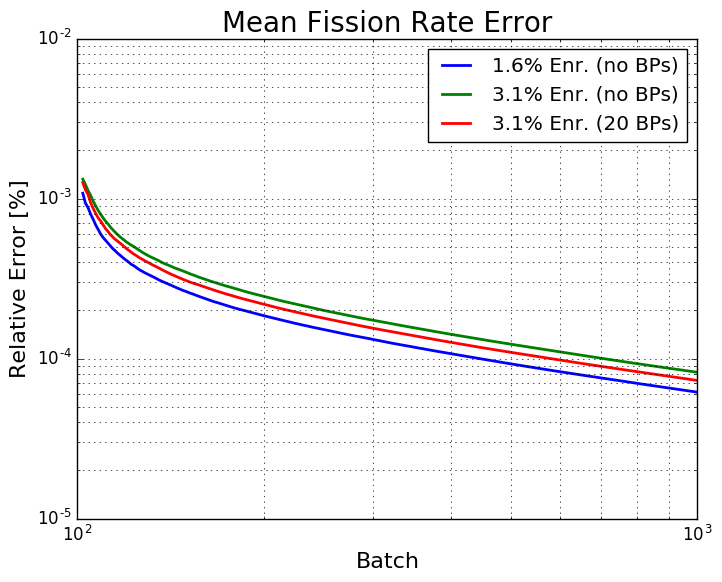
\includegraphics[width=\linewidth]{figures/benchmarks/fission-rates/fiss-conv-mean-assms}
  \caption{}
  \label{fig:chap7-fiss-rate-max-conv-assms}
\end{subfigure}%
\caption[Fission rate error convergence for BEAVRS assemblies]{Fission rate relative error convergence for \ac{BEAVRS} fuel assemblies.}
\label{fig:chap7-fiss-rates-conv-assm}
\end{figure}


%%%%%%%%%%%%%%%%%%%%%%%%%%%%%%%%%%%%%%%%%%%%%
\subsection{U-238 Capture Rate Distributions}
\label{subsec:chap7-capture-rates}

\begin{itemize}[noitemsep]
  \item converged values
  \item convergence by batch
\end{itemize}

\begin{figure}[h!]
\centering
\begin{subfigure}{0.5\textwidth}
  \centering
  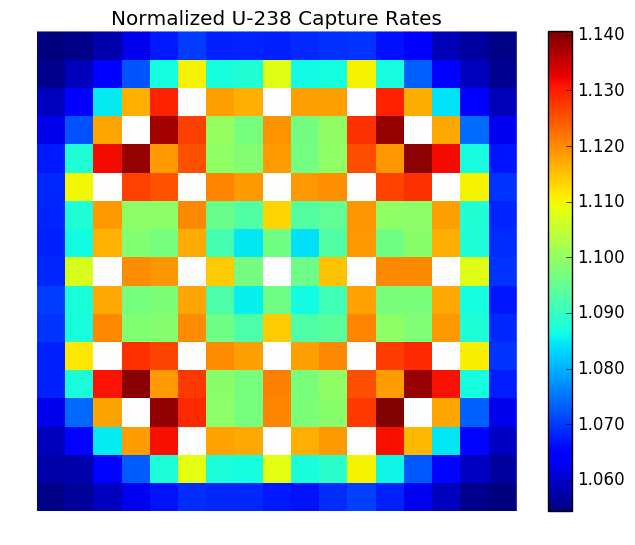
\includegraphics[width=\linewidth]{figures/benchmarks/capture-rates/capt-mean-fuel-16}
  \caption{}
  \label{fig:chap7-capt-rate-mean-1.6-assm}
\end{subfigure}%
\begin{subfigure}{0.5\textwidth}
  \centering
  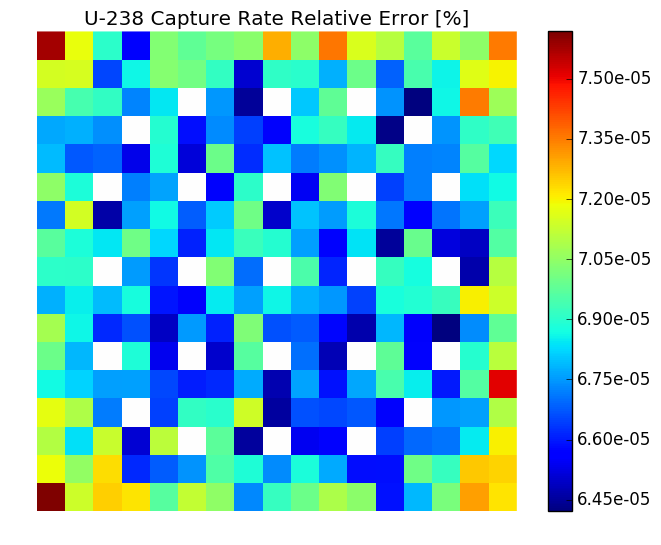
\includegraphics[width=\linewidth]{figures/benchmarks/capture-rates/capt-rel-err-fuel-16}
  \caption{}
  \label{fig:chap7-capt-rate-rel-err-1.6-assm}
\end{subfigure}%
\caption[U-238 capture rates for a 1.6\% enriched assembly]{U-238 capture rates for a 1.6\% enriched assembly.}
\label{fig:chap7-capt-rates-1.6-assm}
\end{figure}

\begin{figure}[h!]
\centering
\begin{subfigure}{0.5\textwidth}
  \centering
  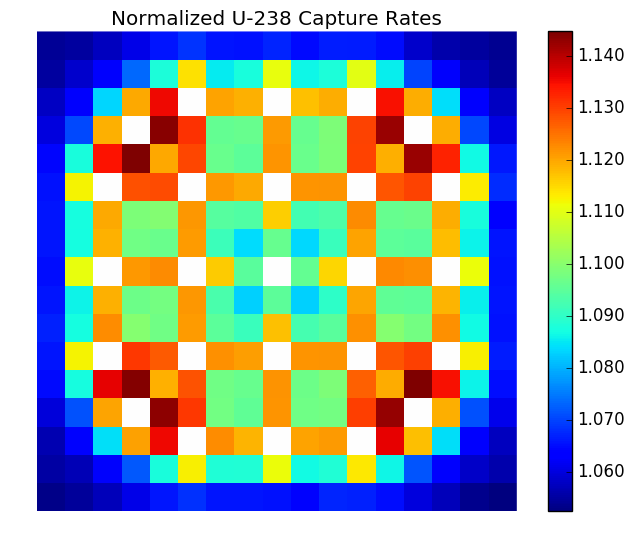
\includegraphics[width=\linewidth]{figures/benchmarks/capture-rates/capt-mean-fuel-31}
  \caption{}
  \label{fig:chap7-capt-rate-mean-3.1-assm}
\end{subfigure}%
\begin{subfigure}{0.5\textwidth}
  \centering
  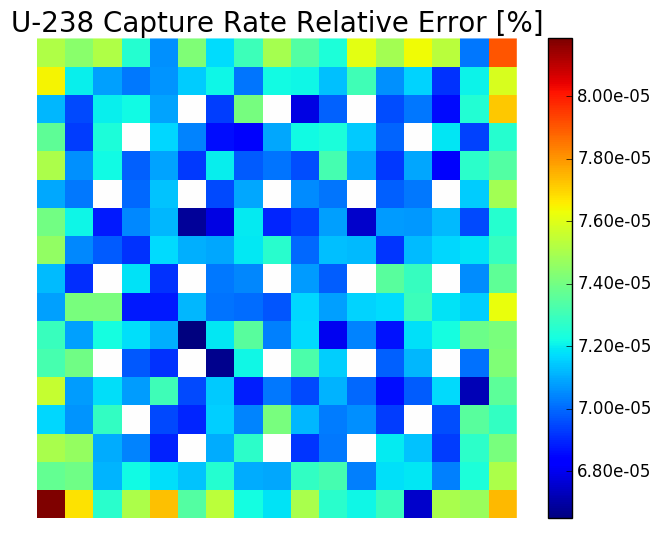
\includegraphics[width=\linewidth]{figures/benchmarks/capture-rates/capt-rel-err-fuel-31}
  \caption{}
  \label{fig:chap7-capt-rate-rel-err-3.1-assm}
\end{subfigure}%
\caption[U-238 capture rates for a 3.1\% enriched assembly]{U-238 capture rates for a 3.1\% enriched assembly.}
\label{fig:chap7-capt-rates-3.1-assm}
\end{figure}

\begin{figure}[h!]
\centering
\begin{subfigure}{0.5\textwidth}
  \centering
  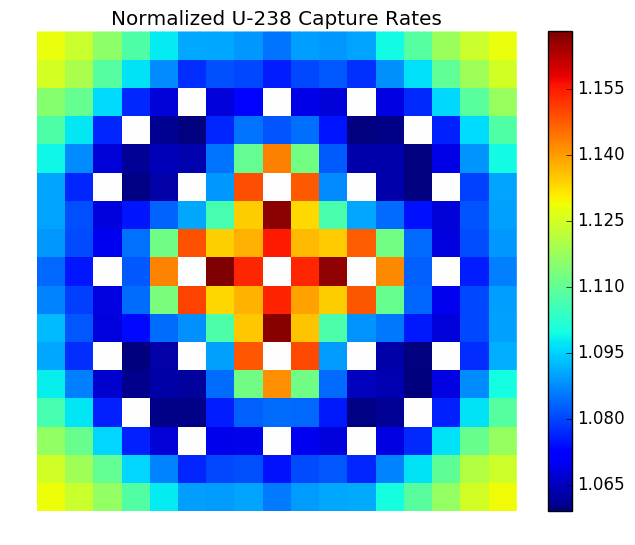
\includegraphics[width=\linewidth]{figures/benchmarks/capture-rates/capt-mean-fuel-31-20BAs}
  \caption{}
  \label{fig:chap7-capt-rate-mean-3.1-20BAs-assm}
\end{subfigure}%
\begin{subfigure}{0.5\textwidth}
  \centering
  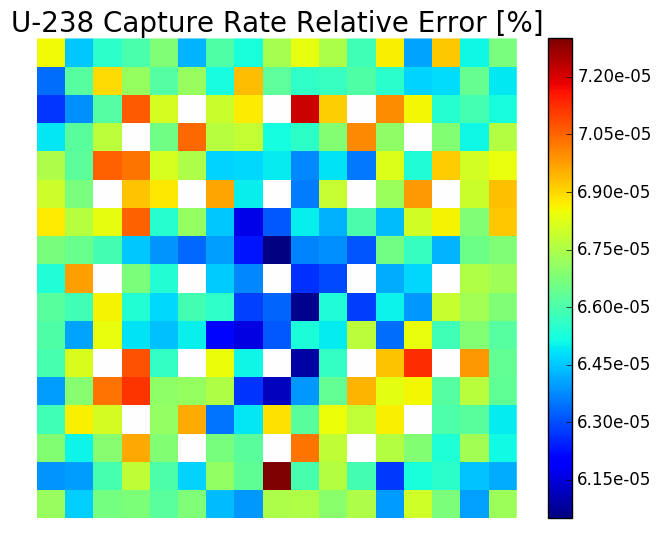
\includegraphics[width=\linewidth]{figures/benchmarks/capture-rates/capt-rel-err-fuel-31-20BAs}
  \caption{}
  \label{fig:chap7-capt-rate-rel-err-3.1-20BAs-assm}
\end{subfigure}%
\caption[U-238 capture rates for a 3.1\% enriched assembly with 20 BPs]{U-238 capture rates for a 3.1\% enriched assembly with 20 \ac{BP}s.}
\label{fig:chap7-capt-rates-3.1-assm-20BAs}
\end{figure}

\begin{figure}[h!]
\centering
\begin{subfigure}{0.5\textwidth}
  \centering
  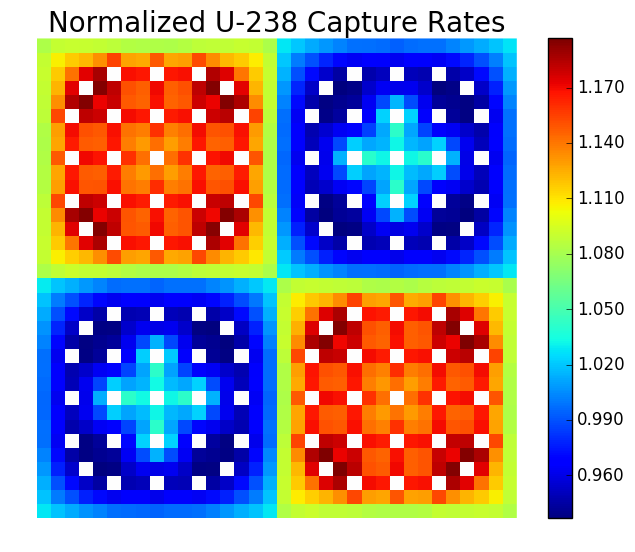
\includegraphics[width=\linewidth]{figures/benchmarks/capture-rates/capt-mean-2x2}
  \caption{}
  \label{fig:chap7-capt-rate-mean-2x2}
\end{subfigure}%
\begin{subfigure}{0.5\textwidth}
  \centering
  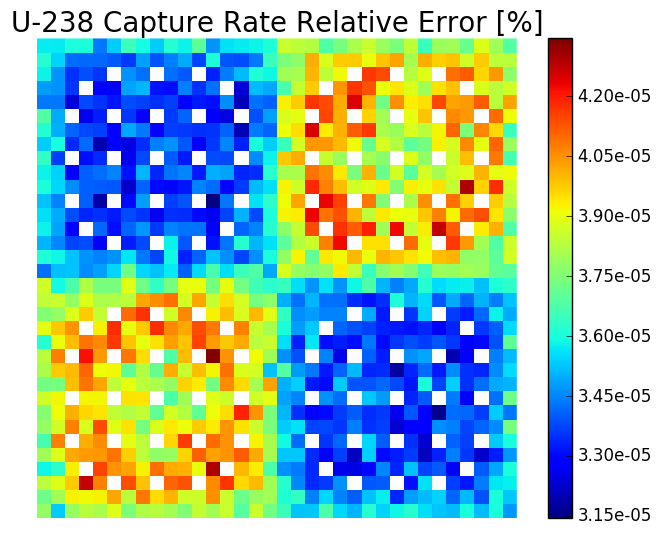
\includegraphics[width=\linewidth]{figures/benchmarks/capture-rates/capt-rel-err-2x2}
  \caption{}
  \label{fig:chap7-capt-rate-rel-err-2x2}
\end{subfigure}%
\caption[U-238 capture rates for a 2$\times$2 colorset]{U-238 capture rates for a 2$\times$2 colorset.}
\label{fig:chap7-capt-rates-2x2}
\end{figure}

\begin{figure}[h!]
\centering
\begin{subfigure}{0.5\textwidth}
  \centering
  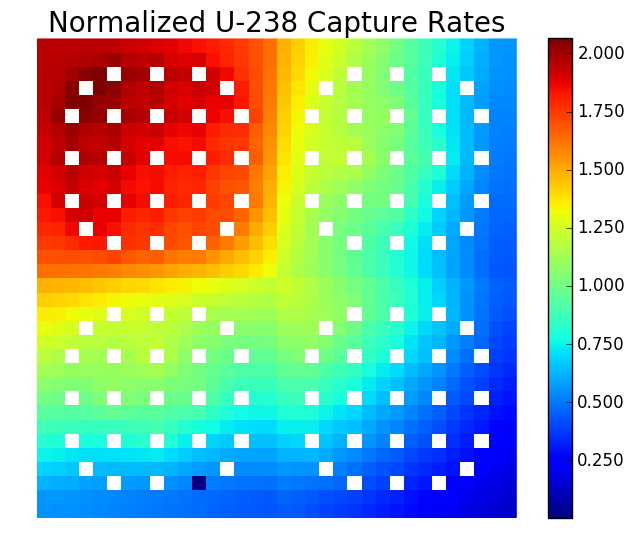
\includegraphics[width=\linewidth]{figures/benchmarks/capture-rates/capt-mean-reflector}
  \caption{}
  \label{fig:chap7-capt-rate-mean-reflector}
\end{subfigure}%
\begin{subfigure}{0.5\textwidth}
  \centering
  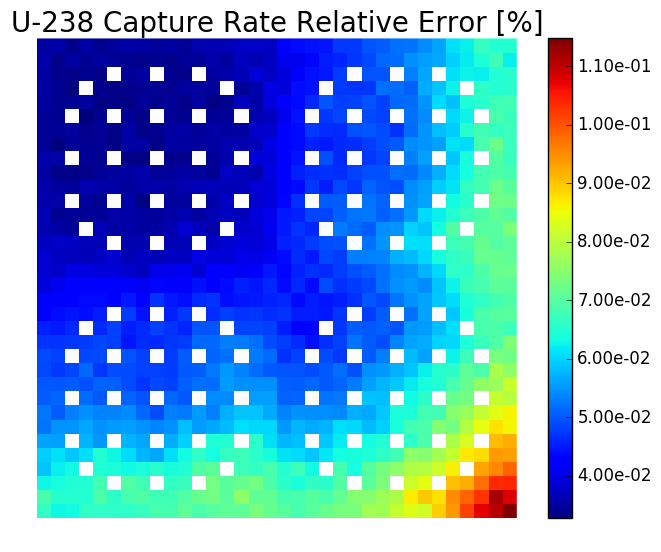
\includegraphics[width=\linewidth]{figures/benchmarks/capture-rates/capt-rel-err-reflector}
  \caption{}
  \label{fig:chap7-capt-rate-rel-err-reflector}
\end{subfigure}%
\caption[U-238 capture rates for a 2$\times$2 colorset with a reflector]{U-238 capture rates for a 2$\times$2 colorset with a reflector.}
\label{fig:chap7-capt-rates-2x2}
\end{figure}

\begin{figure}[h!]
\centering
\begin{subfigure}{0.5\textwidth}
  \centering
  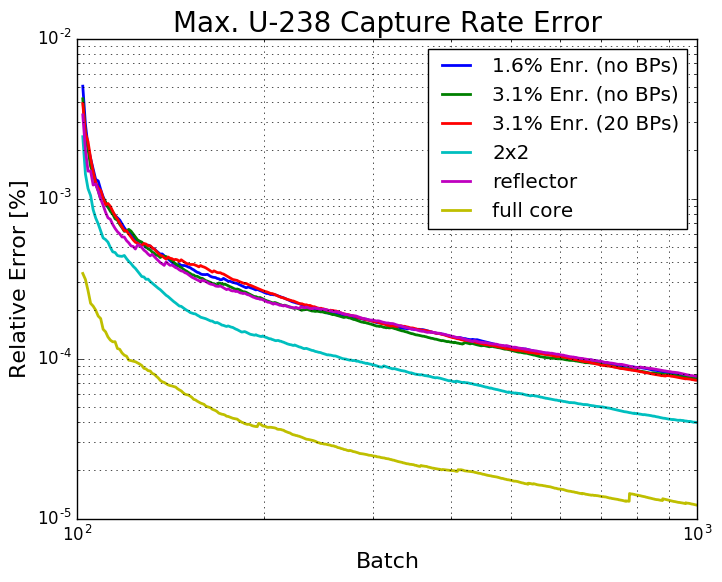
\includegraphics[width=\linewidth]{figures/benchmarks/capture-rates/capt-conv-max-assms}
  \caption{}
  \label{fig:chap7-capt-rate-max-conv-assms}
\end{subfigure}%
\begin{subfigure}{0.5\textwidth}
  \centering
  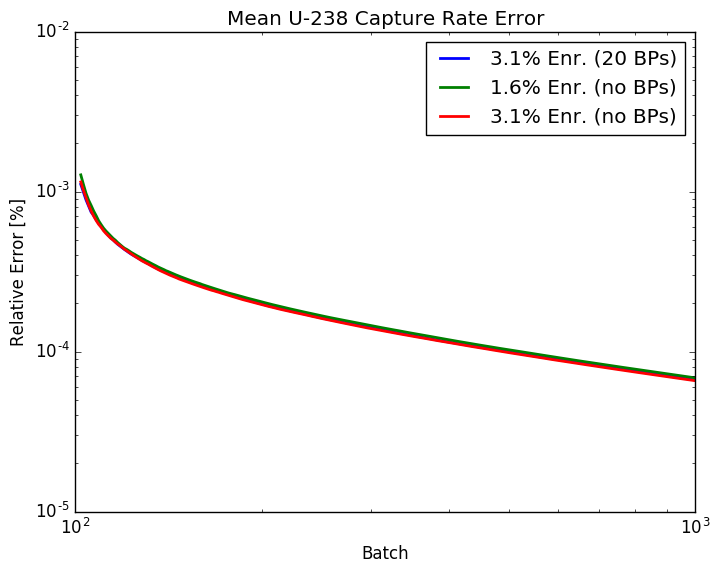
\includegraphics[width=\linewidth]{figures/benchmarks/capture-rates/capt-conv-mean-assms}
  \caption{}
  \label{fig:chap7-capt-rate-max-conv-assms}
\end{subfigure}%
\caption[U-238 capture rate error convergence for BEAVRS assemblies]{U-238 capture rate relative error convergence for \ac{BEAVRS} fuel assemblies.}
\label{fig:chap7-capt-rates-conv-assm}
\end{figure}

%%%%%%%%%%%%%%%%%%%%%%%%%%%%%%%%%%%%%%%%%%%%%%%%%%%%%%%%%%%%%%%%%%%%%%%%%%%%%%%
\section{Convergence Rates}
\label{subsec:chap7-convergence}

\begin{itemize}[noitemsep]
  \item quantify \# histories to $\pm$1 \ac{PCM}
  \item quantify \# histories to $\pm$1\% rel. err.
\end{itemize}